%!TEX root=../main.tex
\section{Empirical analysis} % (fold)
\label{sec:empirical_analysis}

Using simulated data, we compare, in this Section, the behavior of the estimation of the eigencomponents using the diagonalization of the covariance operator and the Gram matrix. The diagonalization of the covariance operator is performed using the methodology of \cite{happMultivariateFunctionalPrincipal2018a}. As this methodology is based on the expansion of each univariate components, we used univariate FPCA if the curves are unidimensional and the FCP-TPA algorithm for regularized tensor decomposition \citep{allenMultiwayFunctionalPrincipal2013a}, if the curves are two-dimensional. We choose to use the FCP-TPA algorithm as it is the one used by \cite{happMultivariateFunctionalPrincipal2018a} in their algorithm and implemented in their software \citep{happ-kurzObjectOrientedSoftwareFunctional2020}. Note that we could also use a two-dimensional basis expansion such as penalized tensor splines or discrete cosine transform, but we do not investigate this expansion here, as we do not want to prespecify a basis of functions.

The results of the simulation are compared using computation times (CT), the integrated squared error (ISE) risk for the multivariate eigenfunctions, the log-absolute error (lAE) risk for the eigenvalues and the mean integreated squared error (MISE) risk for the reconstructed data. Let $\phi_k$ be the true eigenfunction and $\widehat{\phi}_k$ the estimated eigenfunction defined on $\TT{}$. We then defined the ISE as 
\begin{equation}\label{eq:ise_eigenfunctions}
    \text{ISE}(\phi_k, \widehat{\phi}_k) = \normH{\phi_k - \widehat{\phi}_k}^2 = \sum_{p = 1}^P \int_{\TT{p}} \{\phi^{(p)}_k(t_p) - \widehat{\phi}^{(p)}_k(t_p)\}^2 \dd t_p, \quad k = 1, \dots, K.
\end{equation}
Let $\lambda = (\lambda_1, \dots, \lambda_K)$ be the vector of true eigenvalues and $\widehat{\lambda} = (\widehat{\lambda}_1, \dots, \widehat{\lambda}_K)$ be the vector of estimated eigenvalues. We then define the MSE as 
\begin{equation}\label{eq:mse_eigenvalues}
    \log-\text{AE}(\lambda_k, \widehat{\lambda}_k) = \log(\lvert \lambda_k - \widehat{\lambda}_k\rvert), \quad k = 1, \dots, K.
\end{equation}
Let $\mathcal{X}$ be the set of true data and $\widehat{\mathcal{X}}$ be the set of reconstructed data. We defined the MISE of the reconstructed data as
\begin{equation}\label{eq:mise_reconstructed_data}
    \text{MISE}(\mathcal{X}, \widehat{\mathcal{X}}) = \frac{1}{N}\sum_{n = 1}^N \normH{X_n - \widehat{X}_n}^2 = \frac{1}{N}\sum_{n = 1}^N \sum_{p = 1}^P \int_{\TT{p}} \left\{\Xnp(t_p) - \hatXnp(t_p) \right\}^2 \dd t_p.
\end{equation}
Each integral is approximated by the trapezoidal rule with an equidistant grid. Note $\widehat{\phi}$, $\widehat{\lambda}$ and $\widehat{\mathcal{X}}$ the different estimators using the Gram matrix and $\widetilde{\phi}$, $\widetilde{\lambda}$ and $\widetilde{\mathcal{X}}$ the different estimators using the covariance operator. For each configuration $(N, M, P)$, and each of the $500$ samples, we compute the ratios
\begin{equation}
    \frac{\text{ISE}(\phi_k, \widehat{\phi}_k)}{\text{ISE}(\phi_k, \widetilde{\phi}_k)}, \quad \frac{\log -\text{AE}(\lambda_k, \widehat{\lambda}_k)}{\log-\text{AE}(\lambda_k, \widetilde{\lambda}_k)},\quad k = 1, \dots, K, \quad\text{and}\quad \frac{\text{MISE}(\mathcal{X}, \widehat{\mathcal{X}})}{\text{MISE}(\mathcal{X}, \widetilde{\mathcal{X}})},
\end{equation}
and compare them to $1$.

\subsection{Simulation experiments} % (fold)
\label{sub:simulation_experiments}

We consider two simulation scenarios. One consists of multivariate functional data with univariate components defined as unidimensional curves and the other consists of univariate functional data of two-dimensional surfaces. Each experiment is repeated $500$ times.

\begin{scenario}
The simulation setting is based on the simulation in \cite{happMultivariateFunctionalPrincipal2018a}. The data generating process is based on a truncated version of the Karhunen-Loève decomposition. First, we generate a large orthonormal basis $\{\psi_k\}_{1 \leq k \leq K}$ of $\sLp{\TT{}}$ on an interval $\TT{} = [0, T] \subset \RR$. We fix $T_1 = 0$ and $T_{P + 1} = T$ and we generate $P - 1$ cutting points $T_2, \dots, T_P$ uniformly in $\TT{}$ such that $0 = T_1 < \cdots < T_P < T_{P+1} = T$. Let $s_1, \dots, s_P \in \{-1, 1\}$ be coefficients that randomly flip the eigenfunctions. The univariate components of the eigenfunctions are then defined as
\begin{equation}\label{eq:simulation_uni_component}
    \phi_k^{(p)}(t_p) = s_p \restr{\psi_k}{[T_p, T_{p + 1}]}\left(\frac{t_p - T_p}{T_{p + 1} - T_p}\right), \quad k = 1, \dots, K, \quad p = 1, \dots, P.
\end{equation}
The notation $\restr{\phi_k}{[T_p, T_{p + 1}]}$ is the restriction of the function $\phi_k$ to the set $[T_p, T_{p + 1}]$. The set of multivariate functions $\{\psi_k\}_{1 \leq k \leq K}$ is an orthonormal system in $\HH \coloneqq \sLp{\TT{1}} \times \dots \times \sLp{\TT{P}}$ with $\TT{p} = [0, 1]$. Each curve is then simulated using the truncated multivariate Karhunen-Loève expansion \eqref{eq:kl_multi_trunc}:
\begin{equation}
    X(\pointt) = \sum_{k = 1}^K \mathfrak{c}_k \phi_k(\pointt), \quad \pointt \in \TT{},
\end{equation}
where the scores $\mathfrak{c}_k$ are sampled as random normal variables with mean $0$ and variance $\lambda_k$. The eigenvalues $\lambda_k$ are defined with an exponential decrease, $\lambda_k = \exp(-(k + 1)/2)$. We simulate, for each replication of the simulation, $N = 25, 50, 75$ and $100$ observations. Similarly, each component is sampled on a regular grid of $M = 25, 50, 75$ and $100$ sampling points. We compare the methods for $P = 2, 10, 20$ and $50$ components and we set $K = 10$.
\end{scenario}

\begin{scenario}
The data generating process is based on a truncated version of the Karhunen-Loève decomposition. First, we generate an orthonormal basis $\{\phi_k\}_{1 \leq k \leq K}$ of $\sLp{\TT{}}$ on an interval $\TT{} = [0, 1] \times [0, 1]$ as the tensor product of the first Fourier basis functions:
\begin{equation}
    \phi_k(s, t) = \psi_l(s) \otimes \psi_m(t), \quad s, t \in [0, 1],\quad k = 1, \dots, K,
\end{equation}
where $\psi_l$ and $\psi_m$ are elements of the Fourier basis functions.
Each curve is then simulated using the truncated multivariate Karhunen-Loève expansion \eqref{eq:kl_multi_trunc}:
\begin{equation}
    X(s, t) = \sum_{k = 1}^K \mathfrak{c}_k \phi_k(s, t), \quad s, t \in [0, 1],
\end{equation}
where the scores $\mathfrak{c}_k$ are defined as for the Scenario~1. We simulate, for each replication of the simulations, $N = 25, 50, 75$ and $100$ observations. Similarly, each component is sampled on a regular grid of $M = 25 \times 25, 50 \times 50, 75 \times 75$ and $100 \times 100$ sampling points. We set $K = 25$.
\end{scenario}

% subsection simulation_experiments (end)

\subsection{Simulation results} % (fold)
\label{sub:simulation_results}

% Computation time ----------
\begin{results}[Computation time]

Figure~\ref{fig:computation_time_mfd_1d} and Figure~\ref{fig:computation_time_mfd_2d}.

\begin{figure}
     \centering
     \begin{subfigure}[b]{0.49\textwidth}
         \centering
         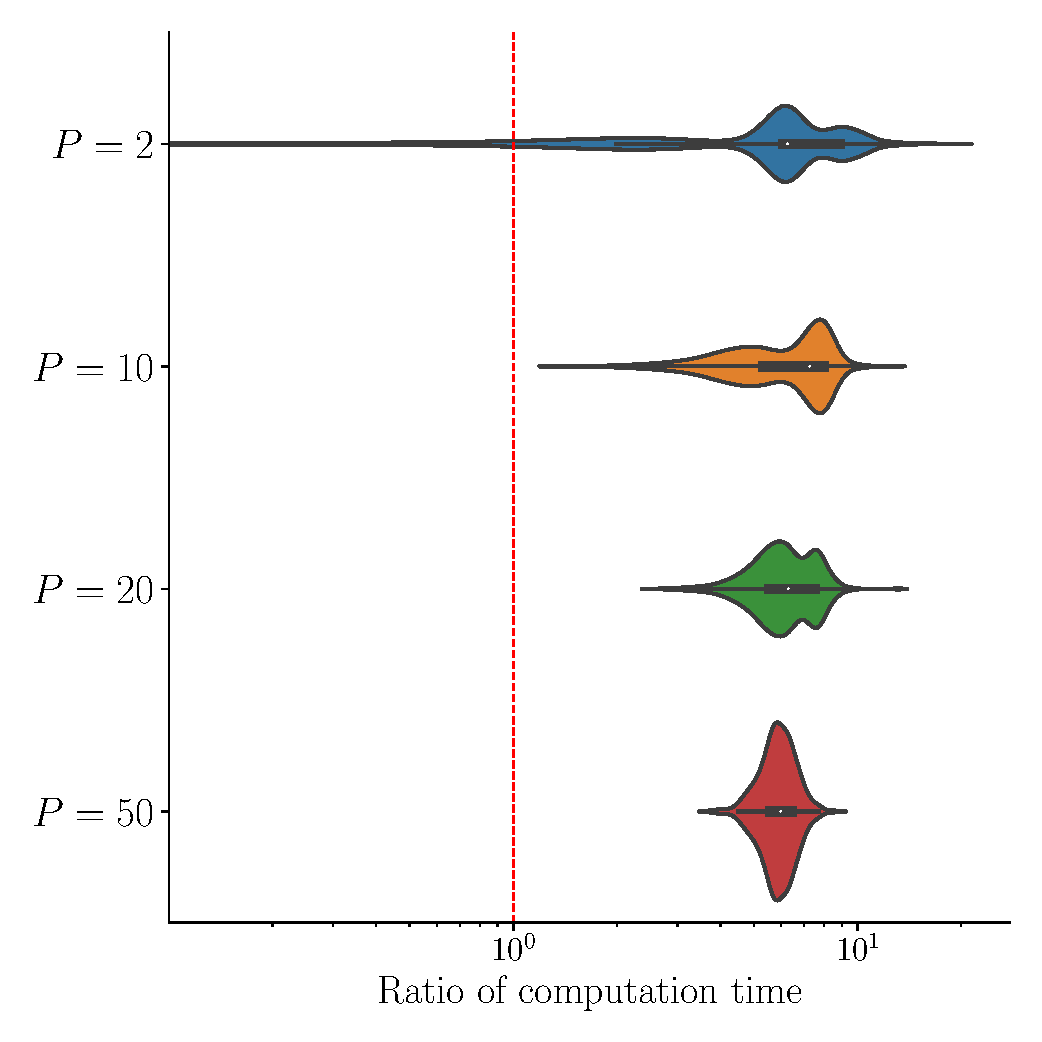
\includegraphics[width=\textwidth]{figures/scenario_1/computation_time_N50_M25.eps}
         \caption{$M = 25$}
         \label{fig:computation_time_mfd_1d_25}
     \end{subfigure}
     \hfill
     \begin{subfigure}[b]{0.49\textwidth}
         \centering
         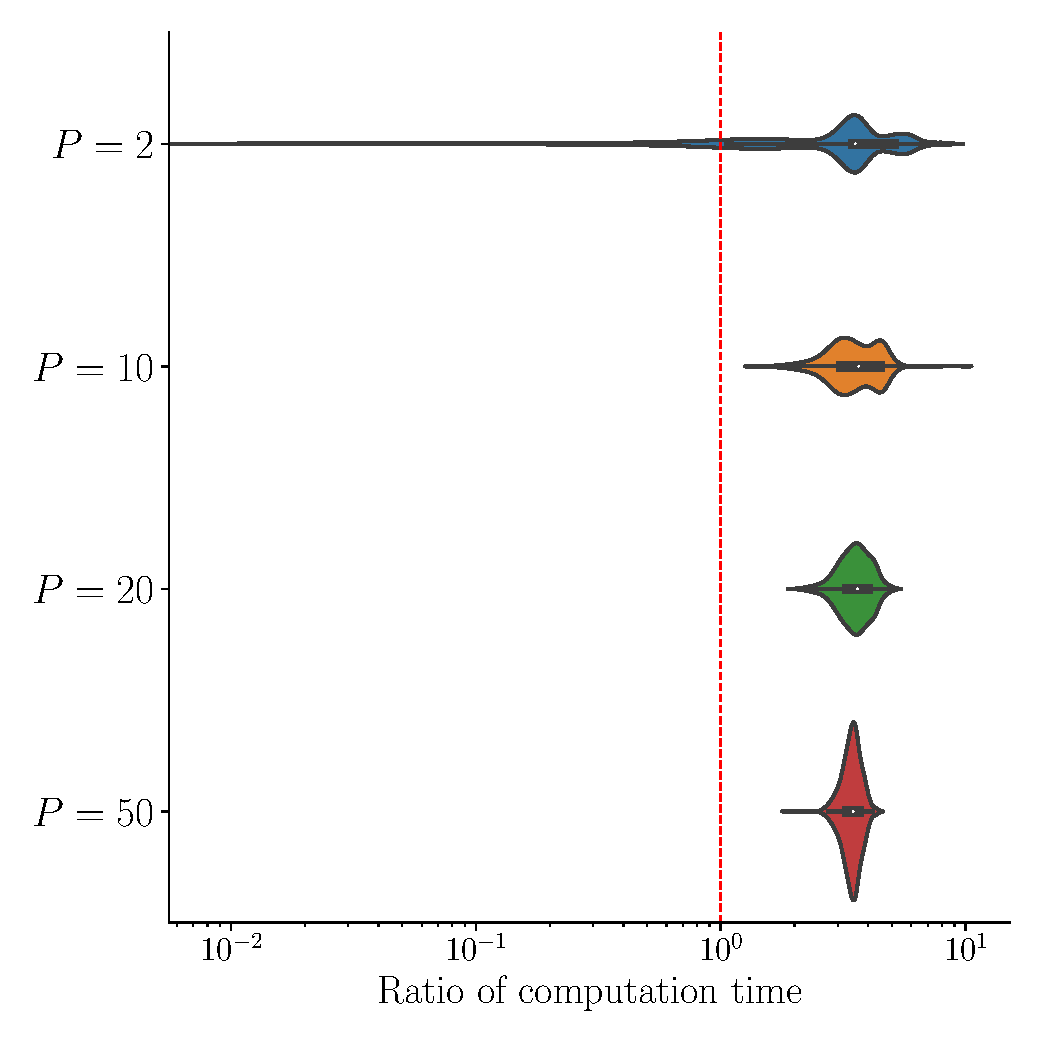
\includegraphics[width=\textwidth]{figures/scenario_1/computation_time_N50_M50.eps}
         \caption{$M = 50$}
         \label{fig:computation_time_mfd_1d_50}
     \end{subfigure}
     \\
     \begin{subfigure}[b]{0.49\textwidth}
         \centering
         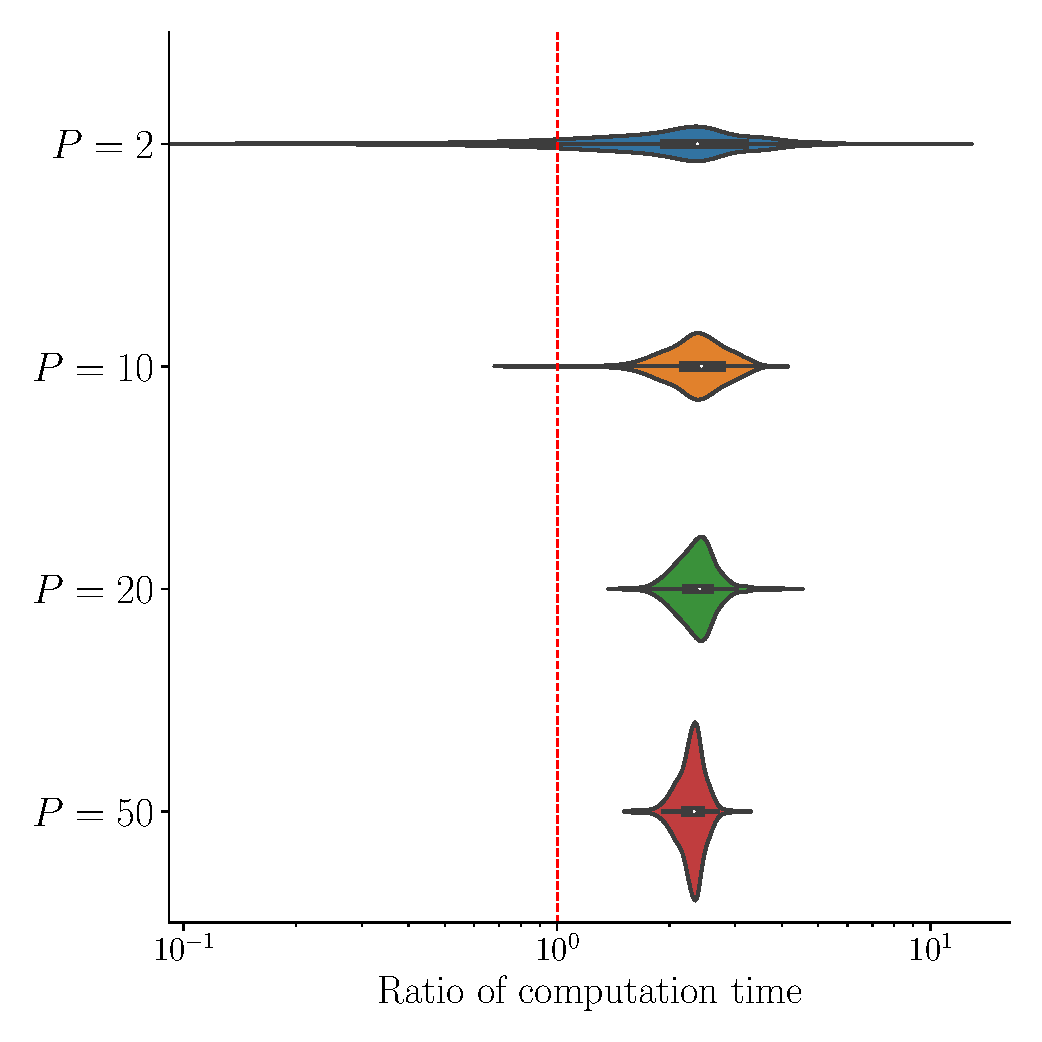
\includegraphics[width=\textwidth]{figures/scenario_1/computation_time_N50_M75.eps}
         \caption{$M = 75$}
         \label{fig:computation_time_mfd_1d_75}
     \end{subfigure}
     \begin{subfigure}[b]{0.49\textwidth}
         \centering
         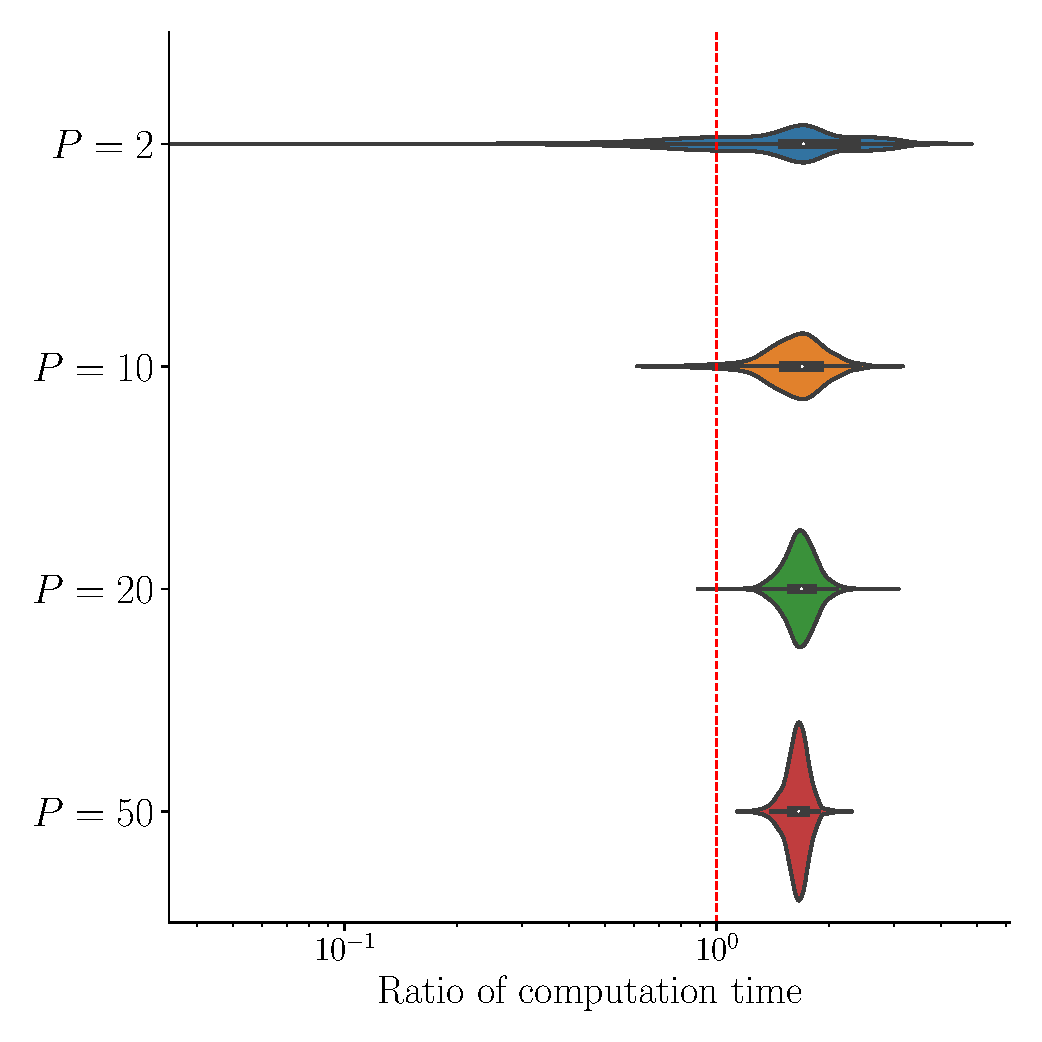
\includegraphics[width=\textwidth]{figures/scenario_1/computation_time_N50_M100.eps}
         \caption{$M = 100$}
         \label{fig:computation_time_mfd_1d_100}
    \end{subfigure}
    \caption{Computation time for multivariate functional data. Each univariate component is defined on a one-dimensional domain. We simulated $N = 50$ observations for each dataset.}
    \label{fig:computation_time_mfd_1d}
\end{figure}

\begin{figure}
     \centering
     \begin{subfigure}[b]{0.49\textwidth}
         \centering
         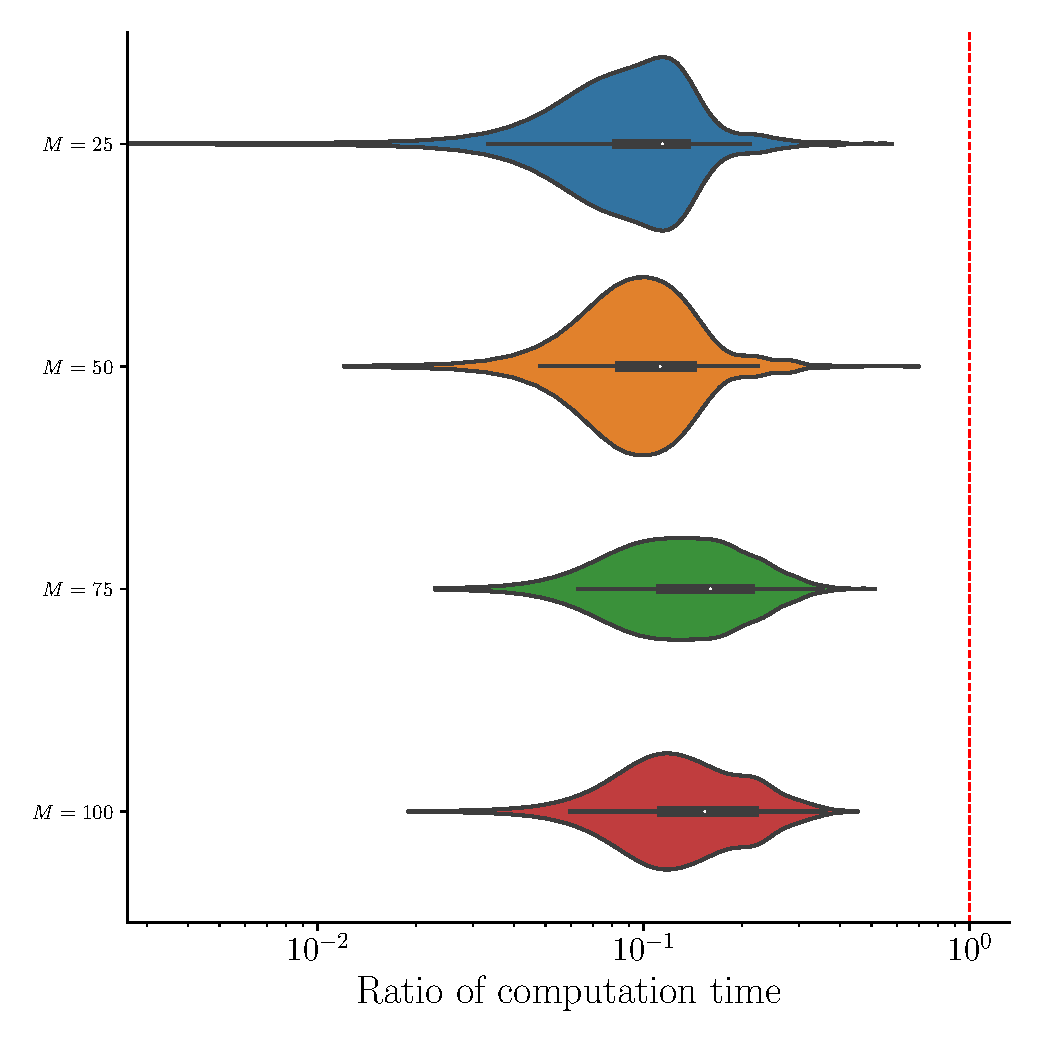
\includegraphics[width=\textwidth]{figures/scenario_2/computation_time_N25.eps}
         \caption{$N = 25$}
         \label{fig:computation_time_mfd_2d_25}
     \end{subfigure}
     \hfill
     \begin{subfigure}[b]{0.49\textwidth}
         \centering
         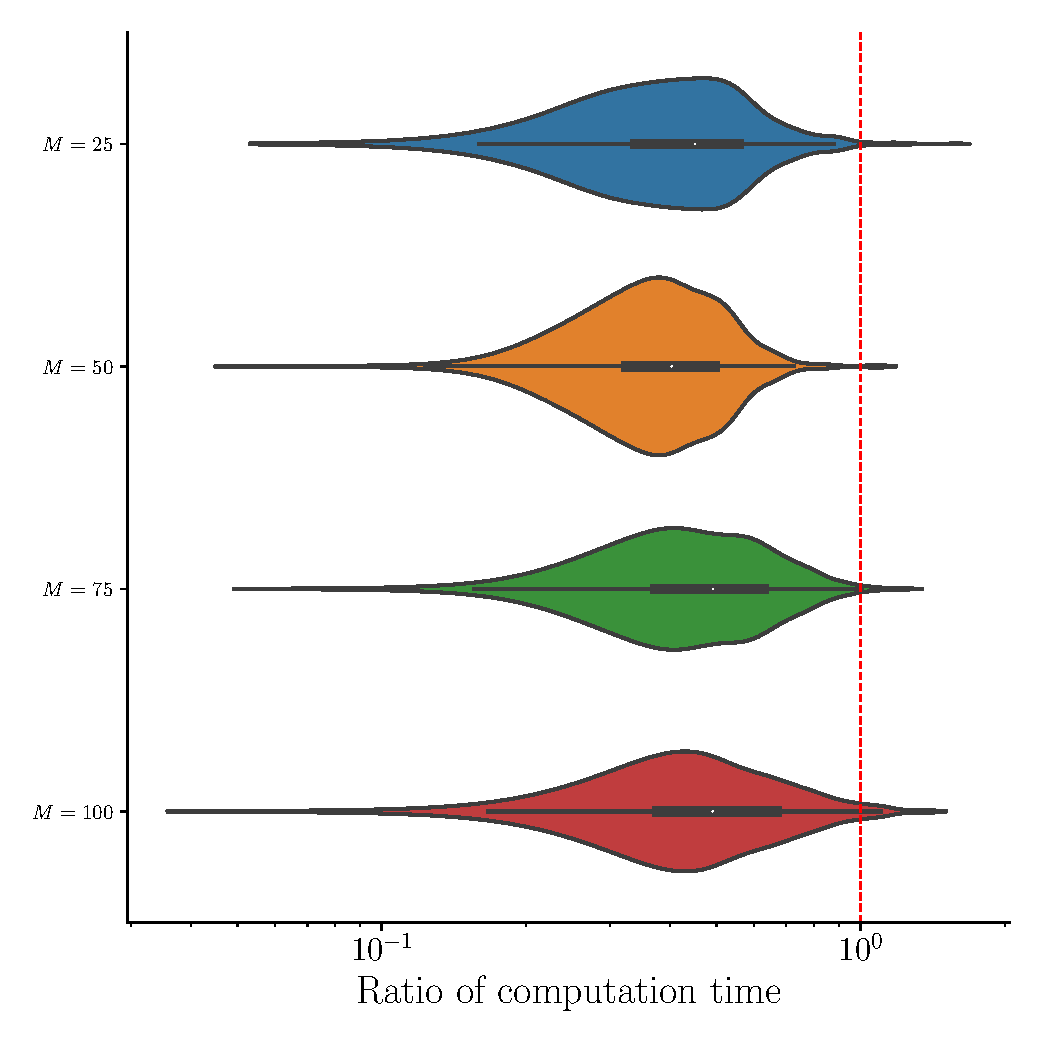
\includegraphics[width=\textwidth]{figures/scenario_2/computation_time_N50.eps}
         \caption{$N = 50$}
         \label{fig:computation_time_mfd_2d_50}
     \end{subfigure}
     \\
     \begin{subfigure}[b]{0.49\textwidth}
         \centering
         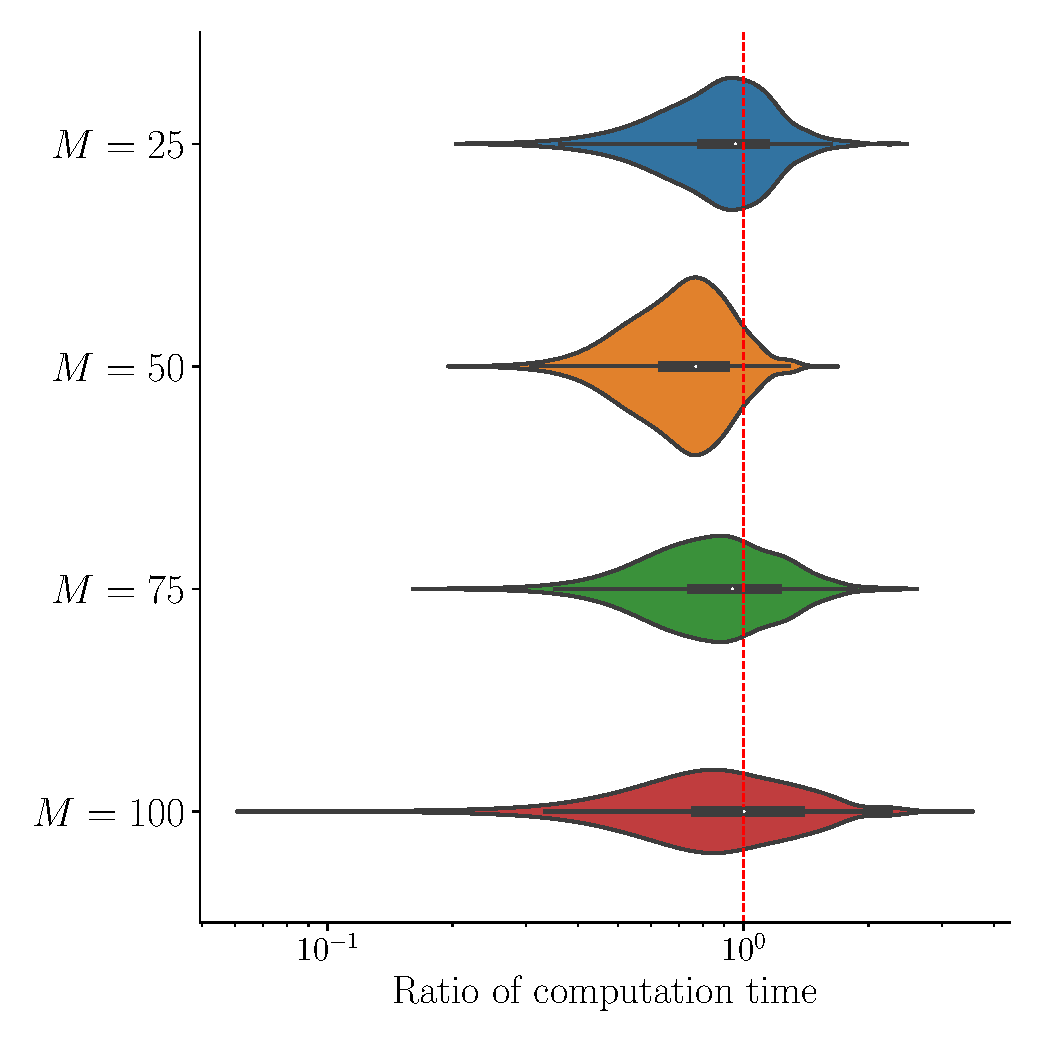
\includegraphics[width=\textwidth]{figures/scenario_2/computation_time_N75.eps}
         \caption{$N = 75$}
         \label{fig:computation_time_mfd_2d_75}
     \end{subfigure}
     \begin{subfigure}[b]{0.49\textwidth}
         \centering
         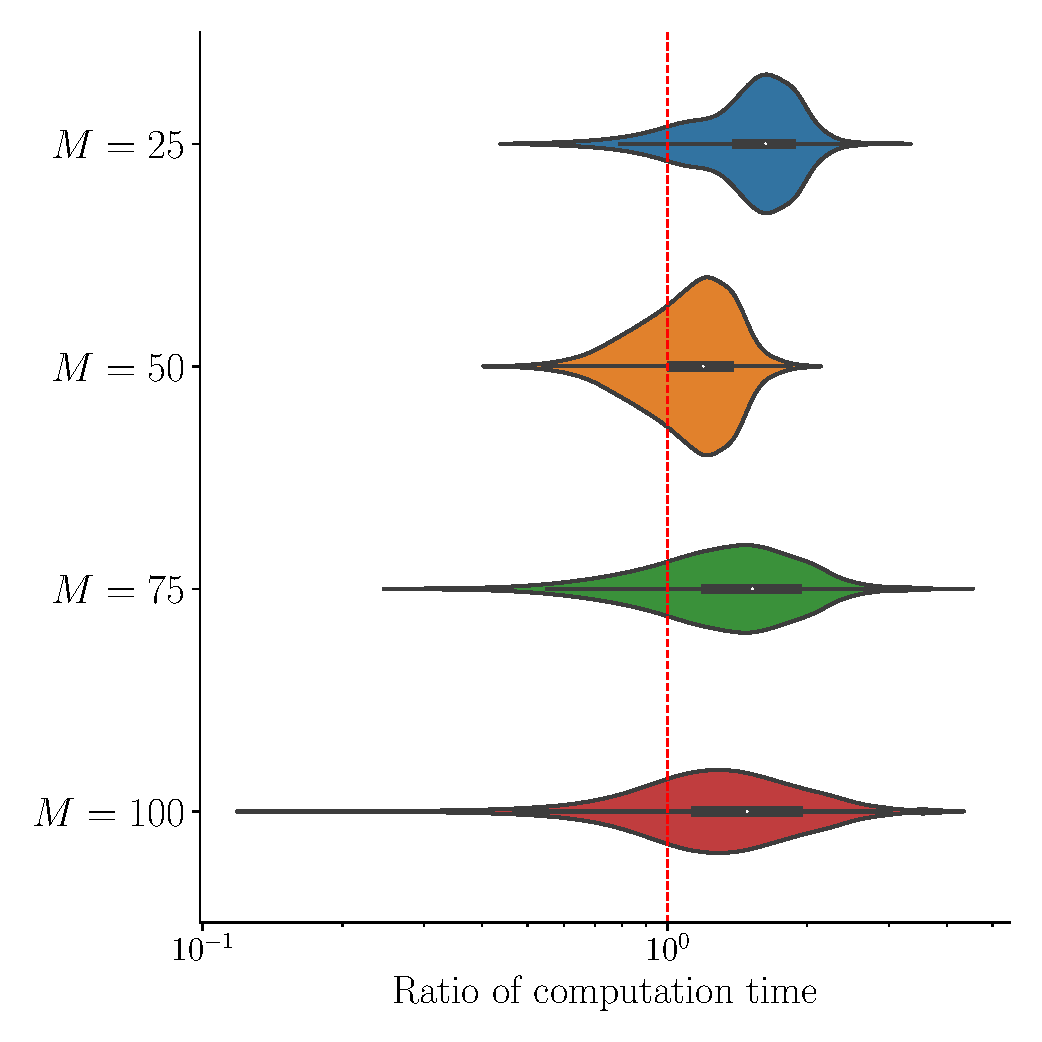
\includegraphics[width=\textwidth]{figures/scenario_2/computation_time_N100.eps}
         \caption{$N = 100$}
         \label{fig:computation_time_mfd_2d_100}
    \end{subfigure}
    \caption{Computation time for univariate functional data of images data}
    \label{fig:computation_time_mfd_2d}
\end{figure}

\end{results}

% Eigenvalues estimation ----------
\begin{results}[Eigenvalues estimation]

Figure~\ref{fig:logAE_mfd_1d} and Figure~\ref{fig:logAE_mfd_2d}.

\begin{figure}
     \centering
     \begin{subfigure}[b]{0.49\textwidth}
         \centering
         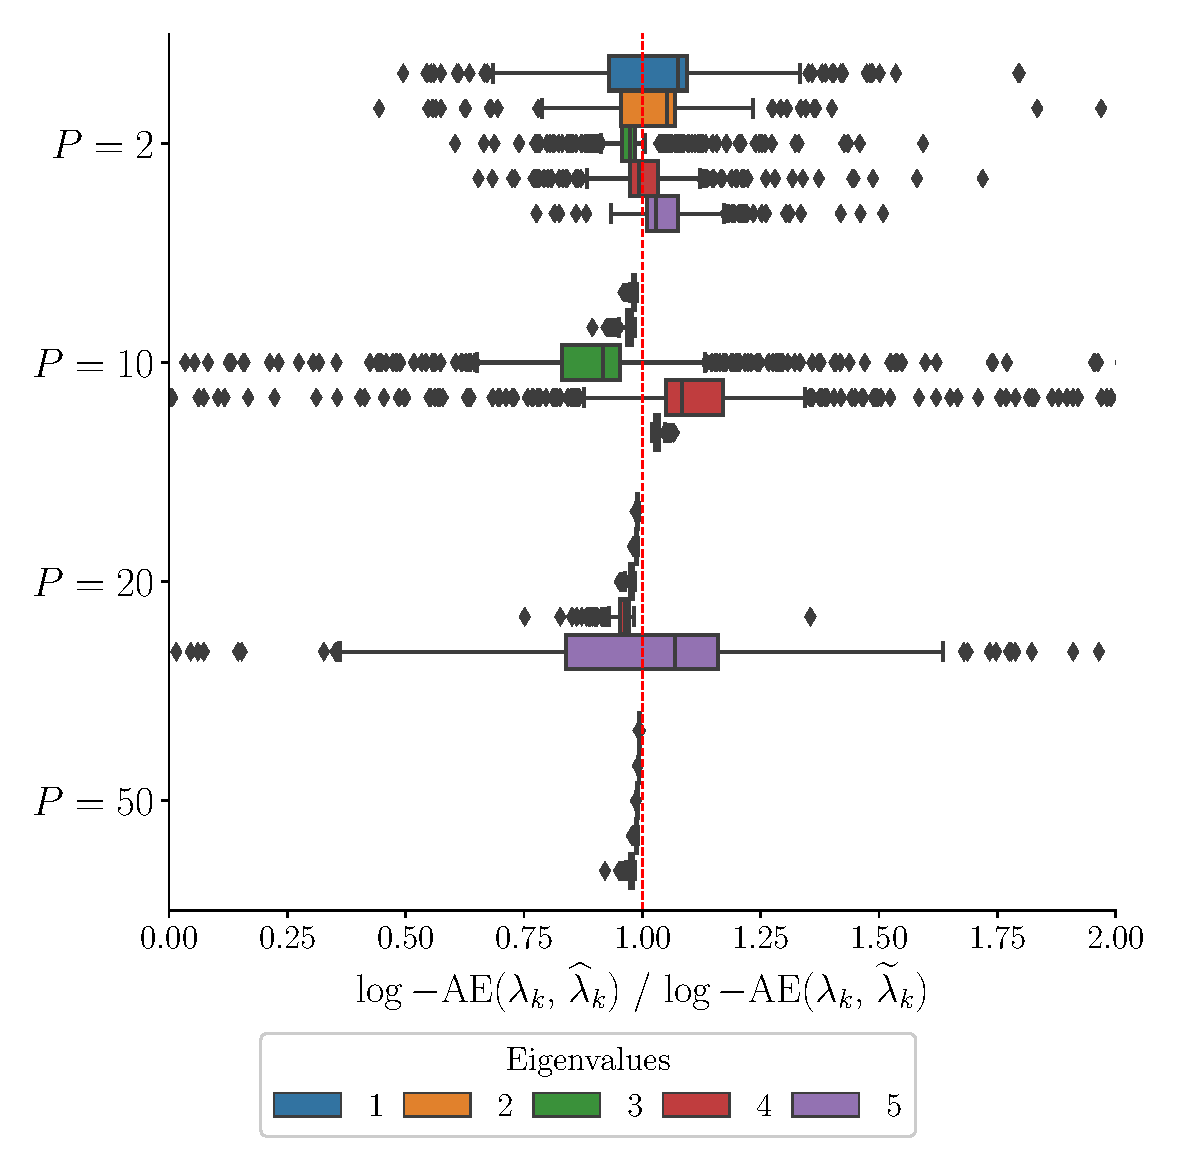
\includegraphics[width=\textwidth]{figures/scenario_1/logAE_N50_M25.eps}
         \caption{$M = 25$}
         \label{fig:logAE_mfd_1d_25}
     \end{subfigure}
     \hfill
     \begin{subfigure}[b]{0.49\textwidth}
         \centering
         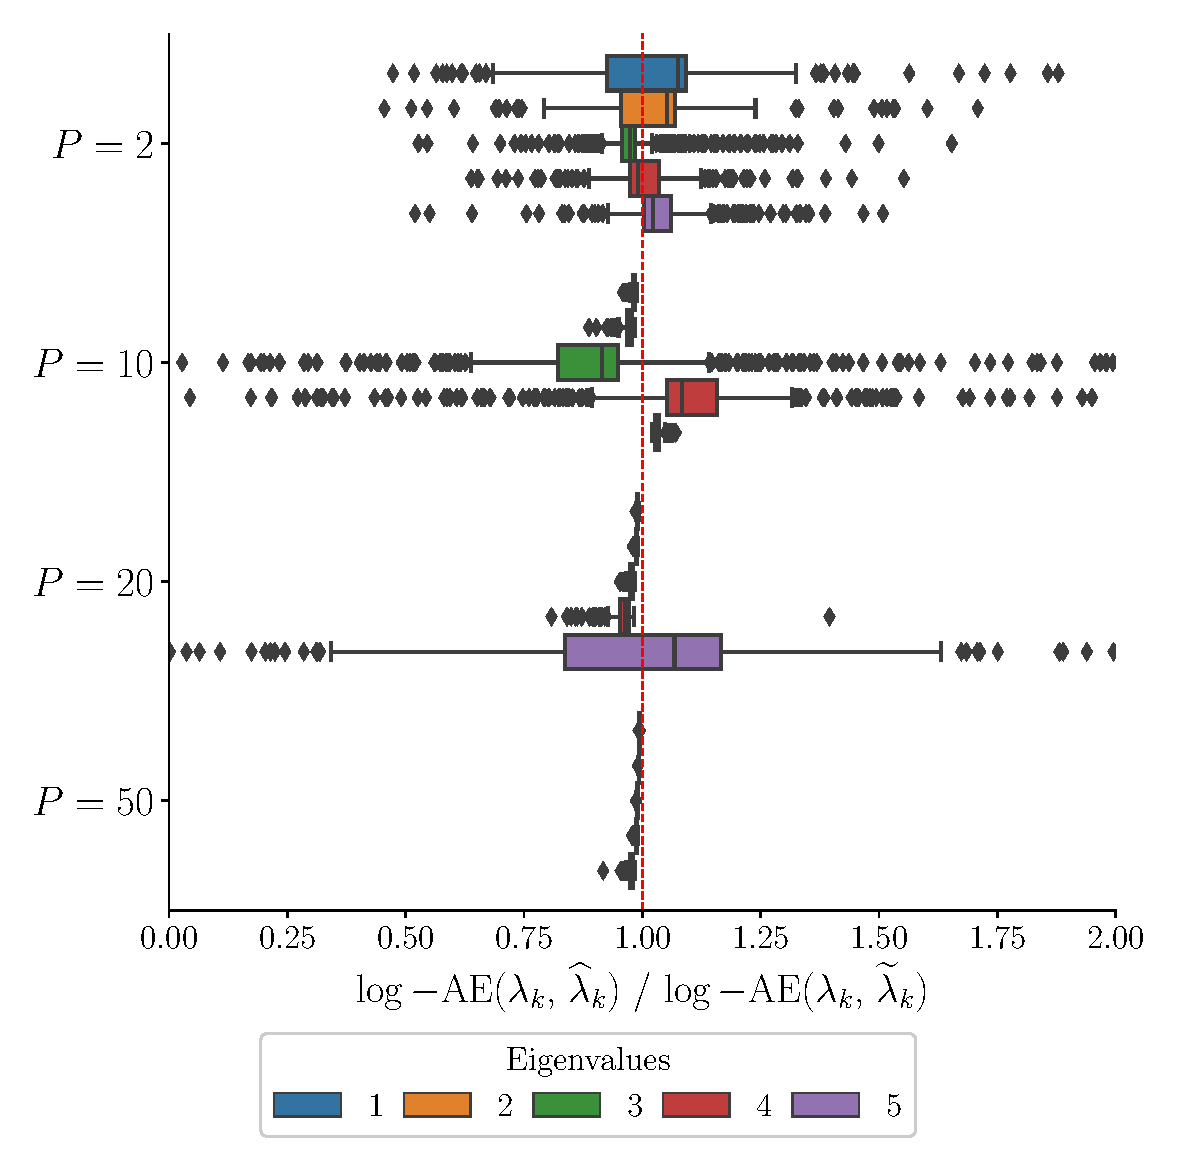
\includegraphics[width=\textwidth]{figures/scenario_1/logAE_N50_M50.eps}
         \caption{$M = 50$}
         \label{fig:logAE_mfd_1d_50}
     \end{subfigure}
     \\
     \begin{subfigure}[b]{0.49\textwidth}
         \centering
         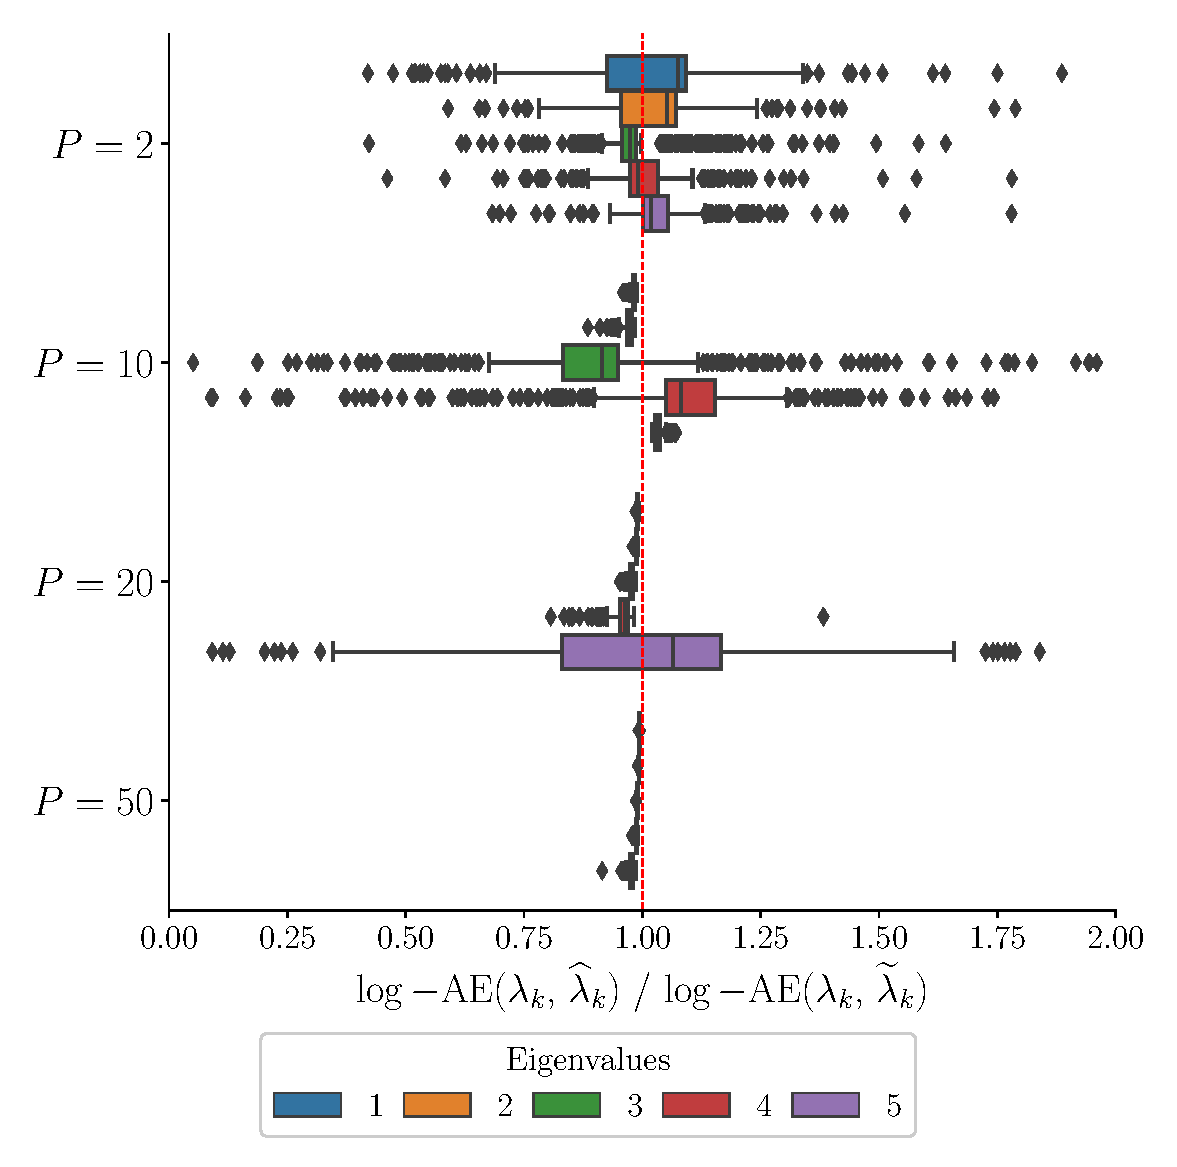
\includegraphics[width=\textwidth]{figures/scenario_1/logAE_N50_M75.eps}
         \caption{$M = 75$}
         \label{fig:logAE_mfd_1d_75}
     \end{subfigure}
     \begin{subfigure}[b]{0.49\textwidth}
         \centering
         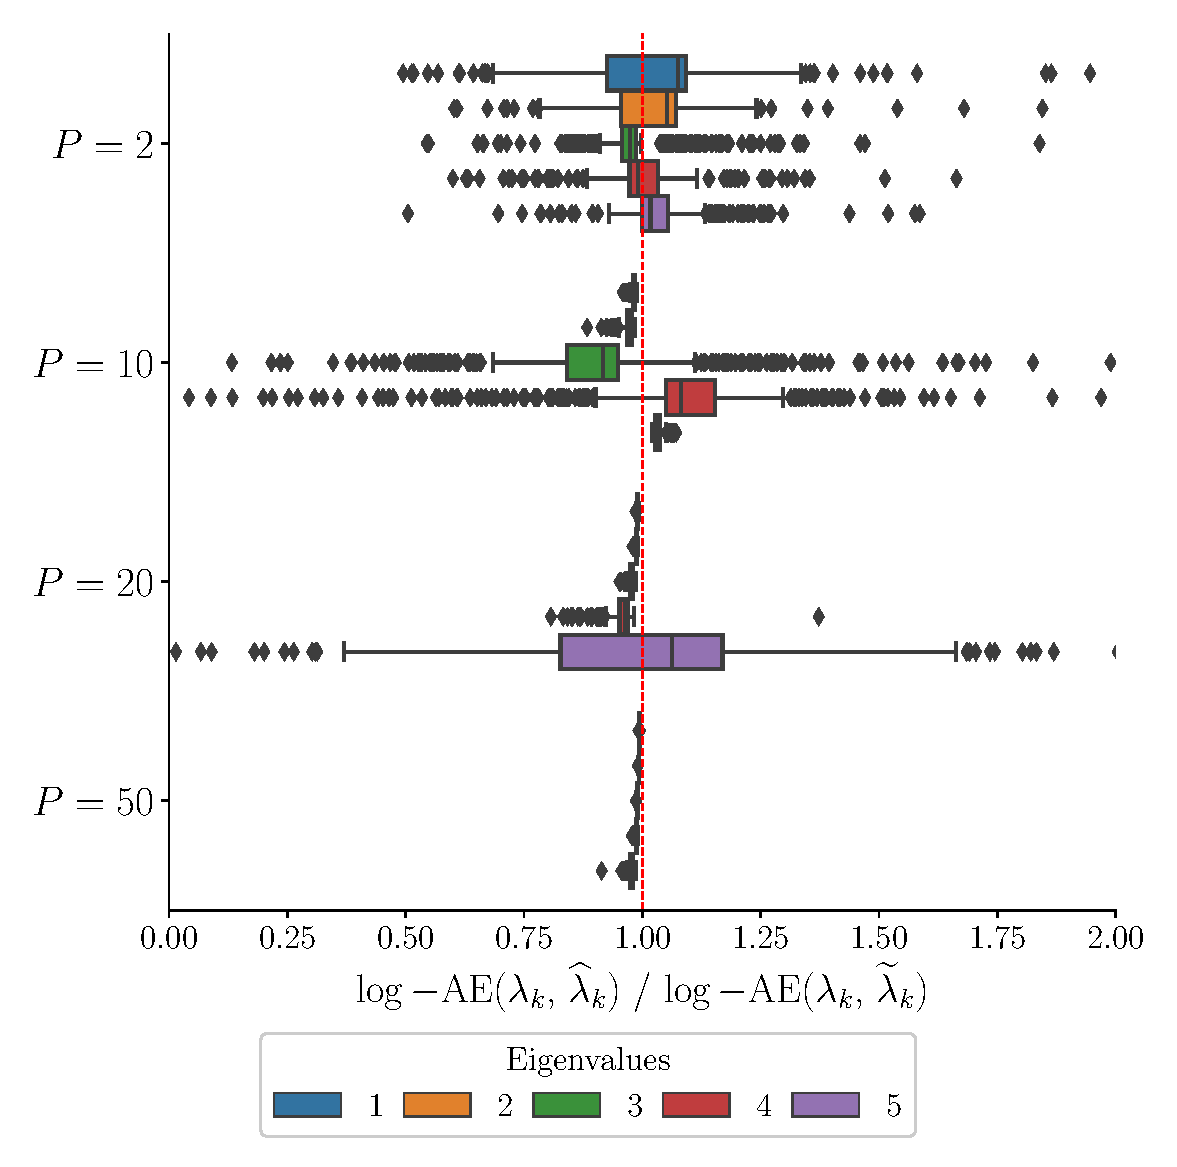
\includegraphics[width=\textwidth]{figures/scenario_1/logAE_N50_M100.eps}
         \caption{$M = 100$}
         \label{fig:logAE_mfd_1d_100}
    \end{subfigure}
    \caption{$\log-$AE for multivariate functional data. Each univariate component is defined on a one-dimensional domain. We simulated $N = 50$ observations for each dataset.}
    \label{fig:logAE_mfd_1d}
\end{figure}

\begin{figure}
     \centering
     \begin{subfigure}[b]{0.49\textwidth}
         \centering
         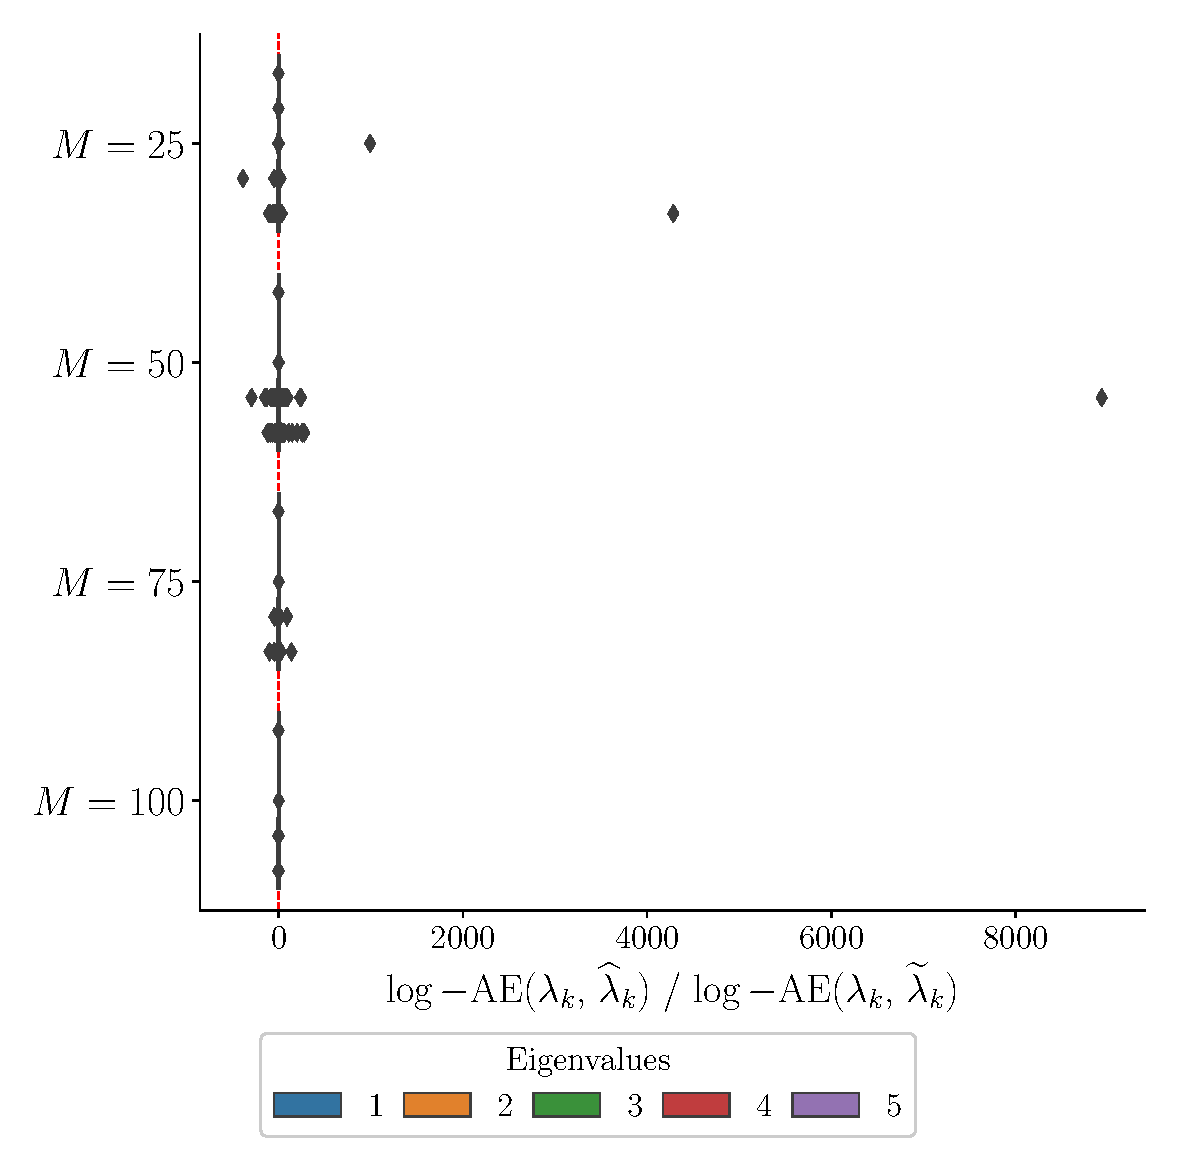
\includegraphics[width=\textwidth]{figures/scenario_2/logAE_N25.eps}
         \caption{$N = 25$}
         \label{fig:logAE_mfd_2d_25}
     \end{subfigure}
     \hfill
     \begin{subfigure}[b]{0.49\textwidth}
         \centering
         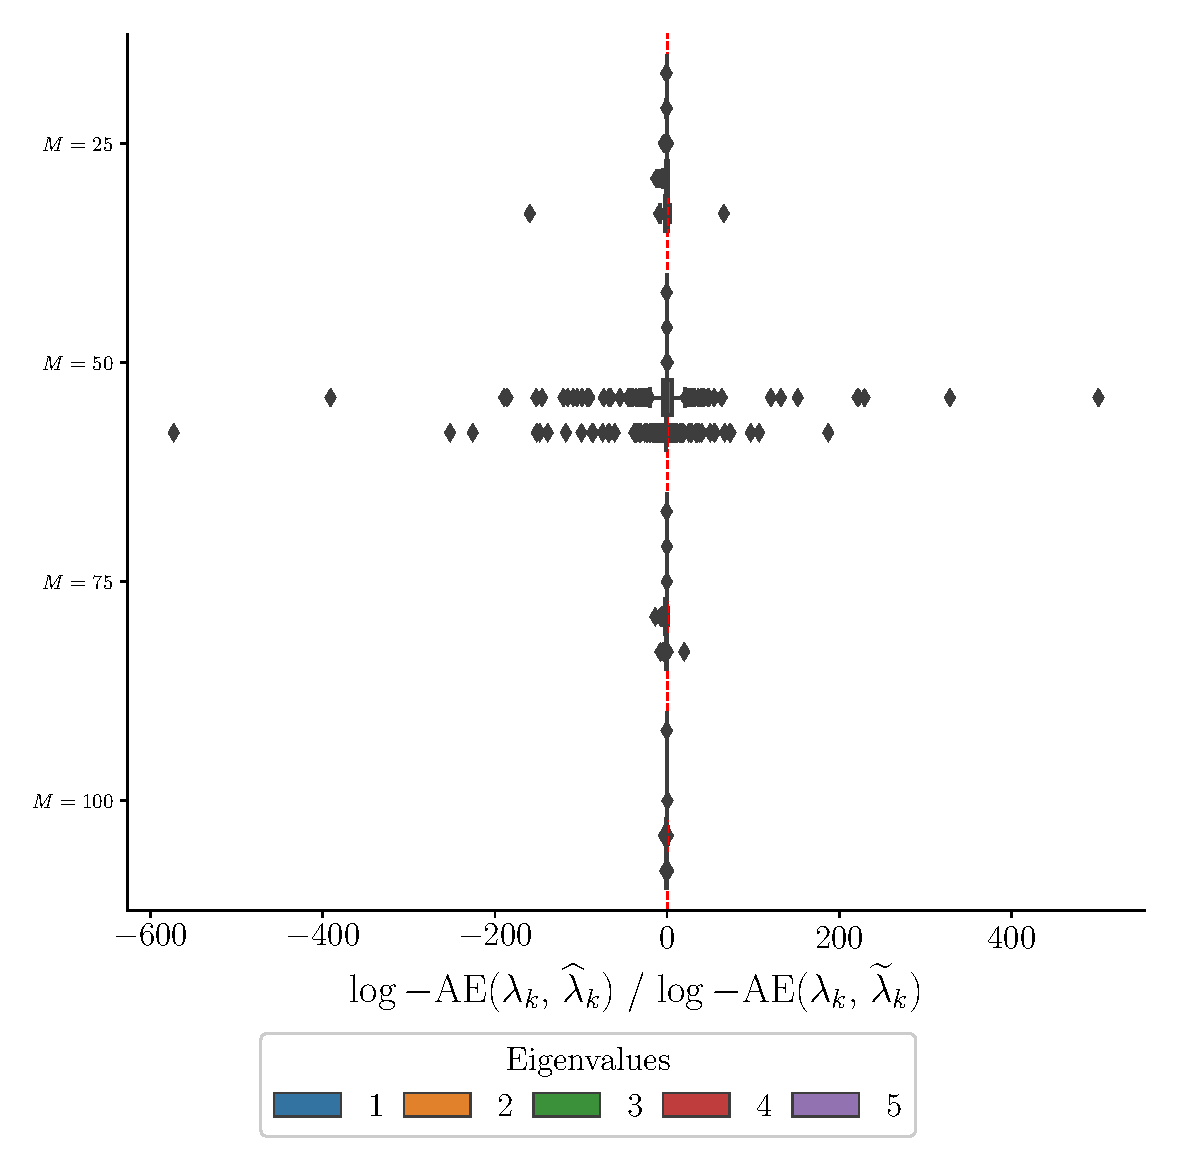
\includegraphics[width=\textwidth]{figures/scenario_2/logAE_N50.eps}
         \caption{$N = 50$}
         \label{fig:logAE_mfd_2d_50}
     \end{subfigure}
     \\
     \begin{subfigure}[b]{0.49\textwidth}
         \centering
         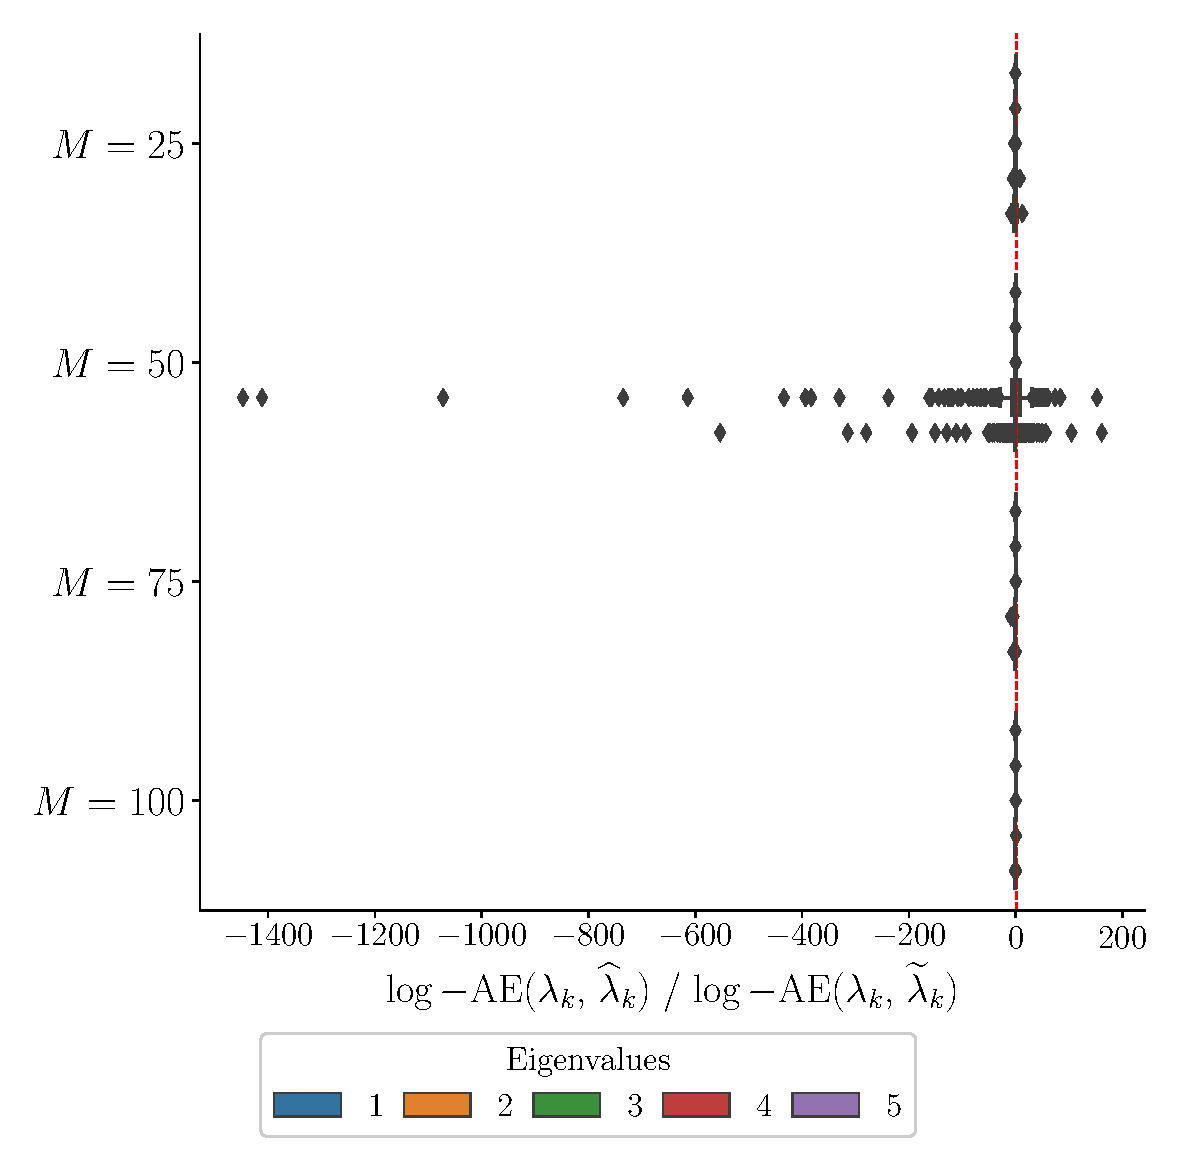
\includegraphics[width=\textwidth]{figures/scenario_2/logAE_N75.eps}
         \caption{$N = 75$}
         \label{fig:logAE_mfd_2d_75}
     \end{subfigure}
     \begin{subfigure}[b]{0.49\textwidth}
         \centering
         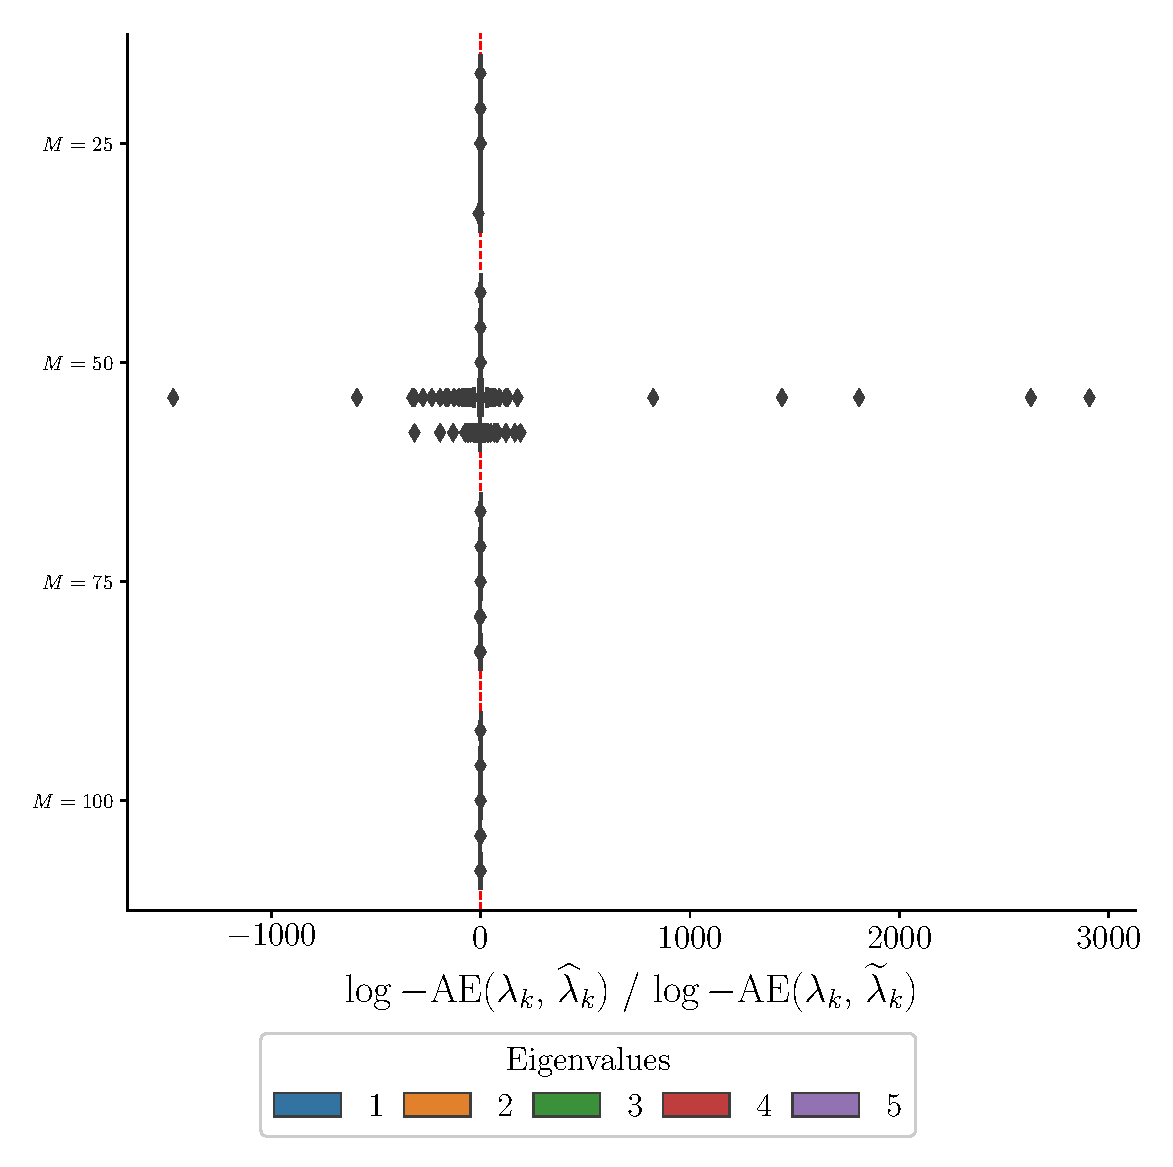
\includegraphics[width=\textwidth]{figures/scenario_2/logAE_N100.eps}
         \caption{$N = 100$}
         \label{fig:logAE_mfd_2d_100}
    \end{subfigure}
    \caption{$\log-$AE for univariate functional data of images data}
    \label{fig:logAE_mfd_2d}
\end{figure}

\end{results}

% Eigenfunctions estimation ----------
\begin{results}[Eigenfunctions estimation]

Figure~\ref{fig:ise_mfd_1d} and Figure~\ref{fig:ise_mfd_2d}.

\begin{figure}
     \centering
     \begin{subfigure}[b]{0.49\textwidth}
         \centering
         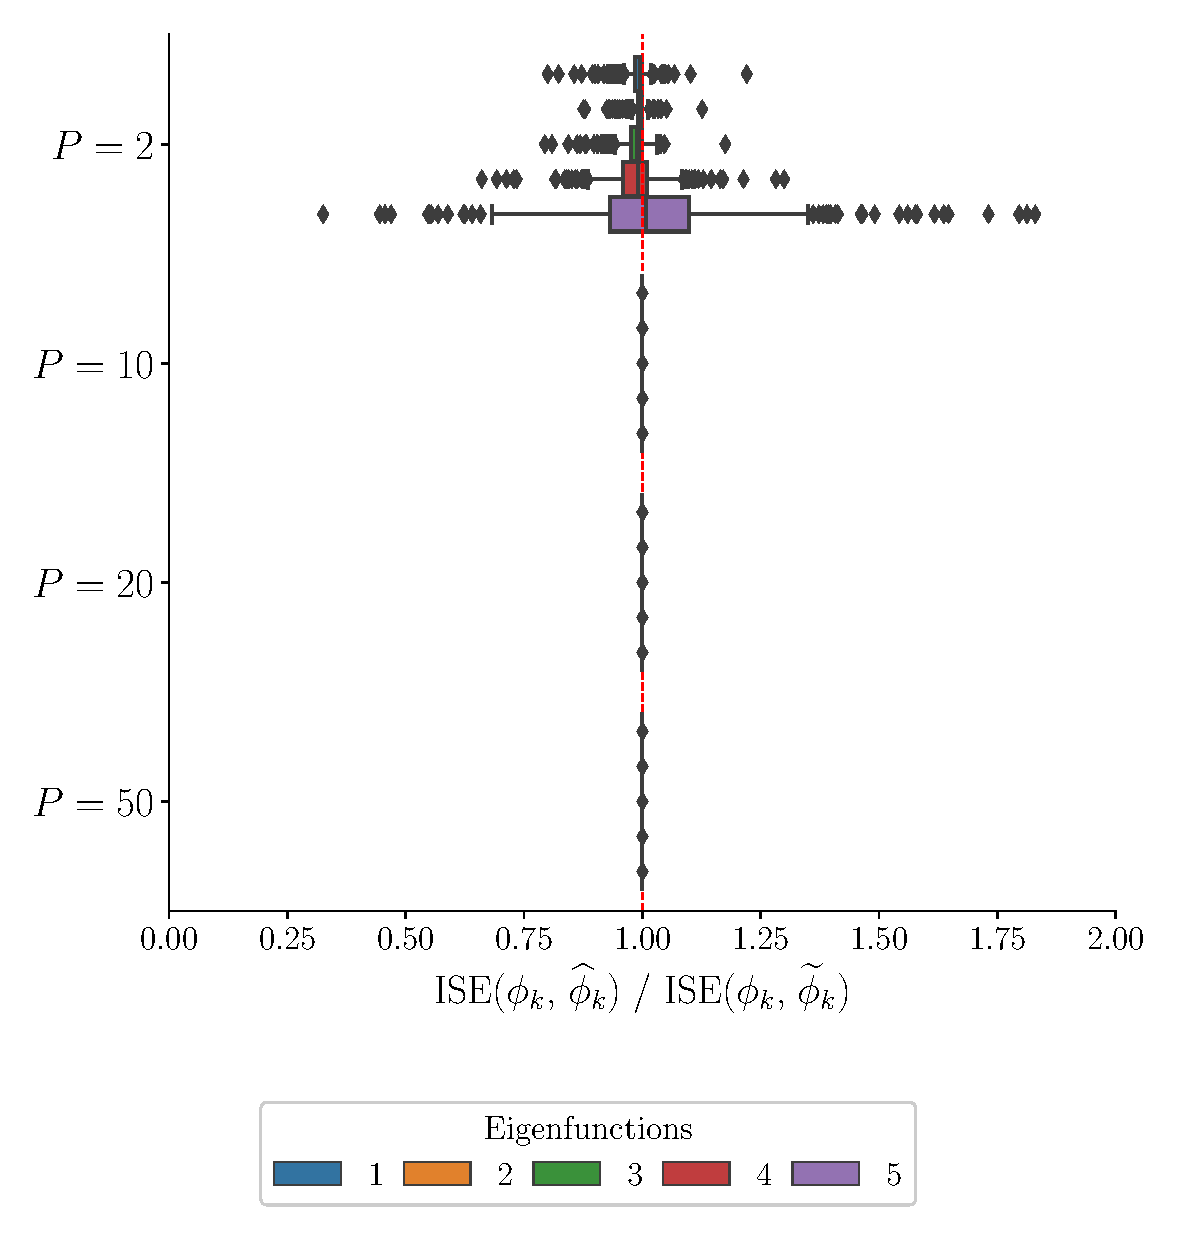
\includegraphics[width=\textwidth]{figures/scenario_1/ise_N50_M25.eps}
         \caption{$M = 25$}
         \label{fig:ise_mfd_1d_25}
     \end{subfigure}
     \hfill
     \begin{subfigure}[b]{0.49\textwidth}
         \centering
         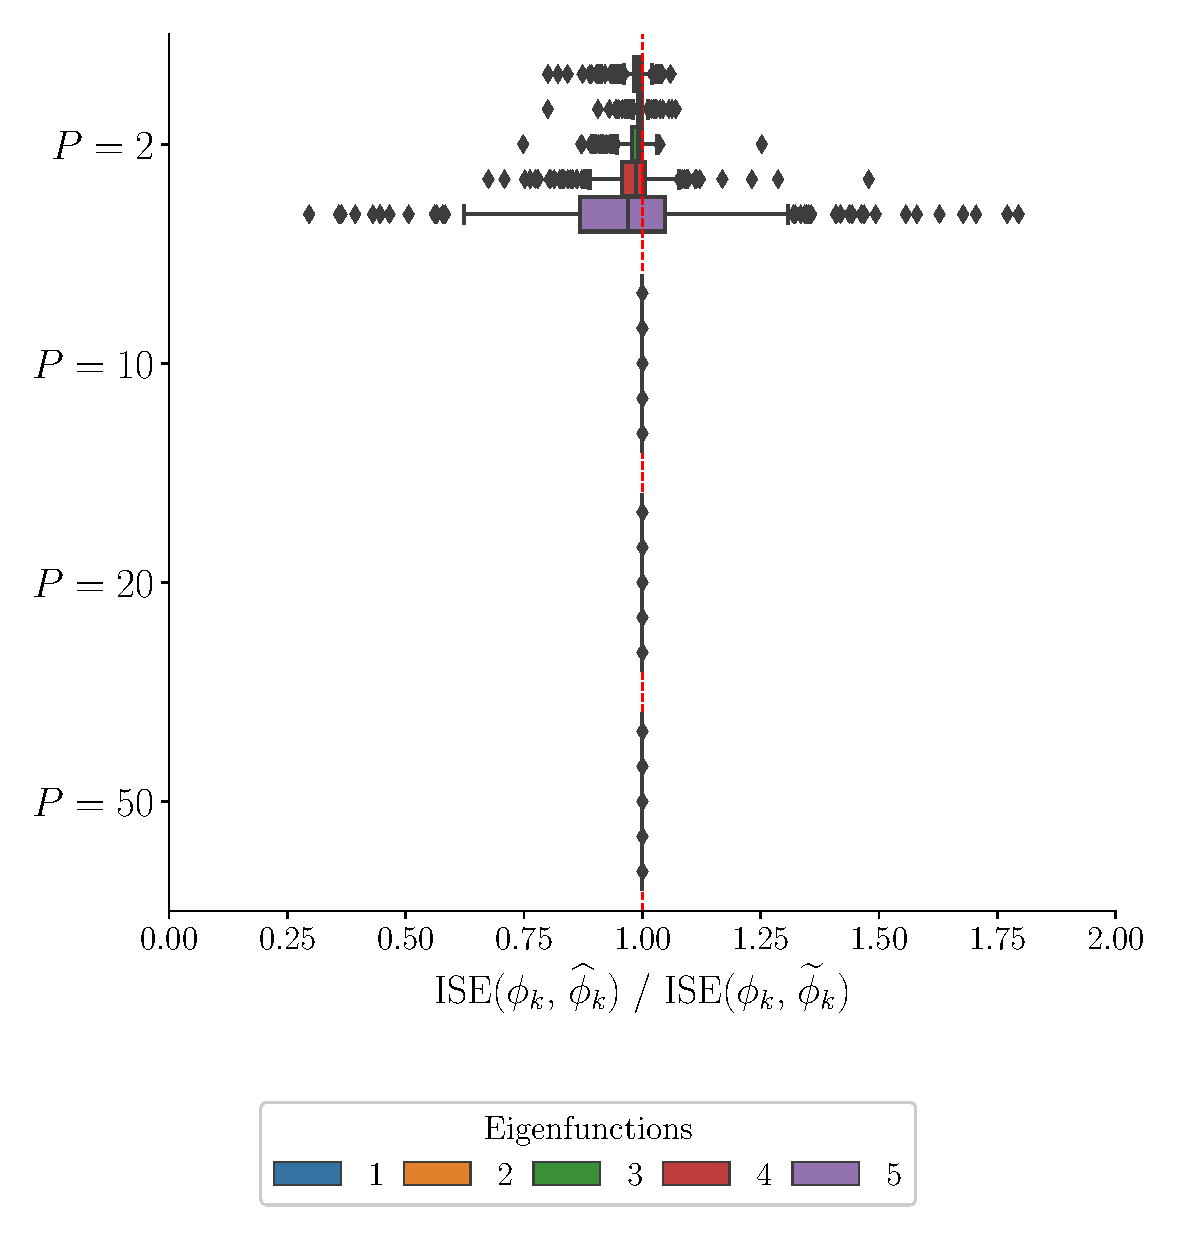
\includegraphics[width=\textwidth]{figures/scenario_1/ise_N50_M50.eps}
         \caption{$M = 50$}
         \label{fig:ise_mfd_1d_50}
     \end{subfigure}
     \\
     \begin{subfigure}[b]{0.49\textwidth}
         \centering
         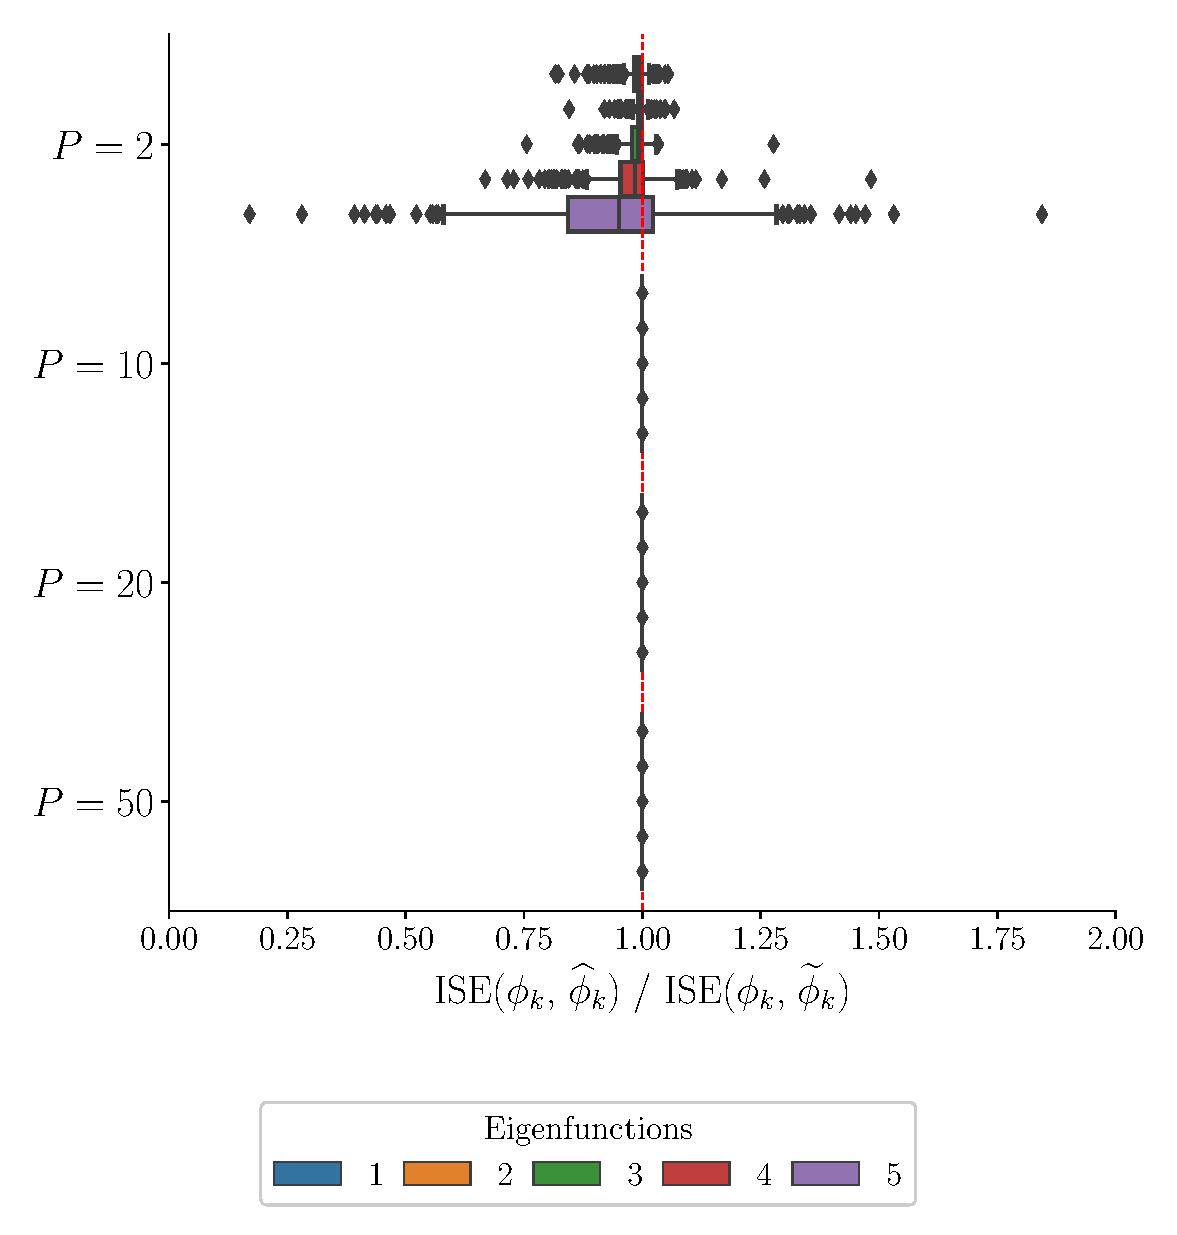
\includegraphics[width=\textwidth]{figures/scenario_1/ise_N50_M75.eps}
         \caption{$M = 75$}
         \label{fig:ise_mfd_1d_75}
     \end{subfigure}
     \begin{subfigure}[b]{0.49\textwidth}
         \centering
         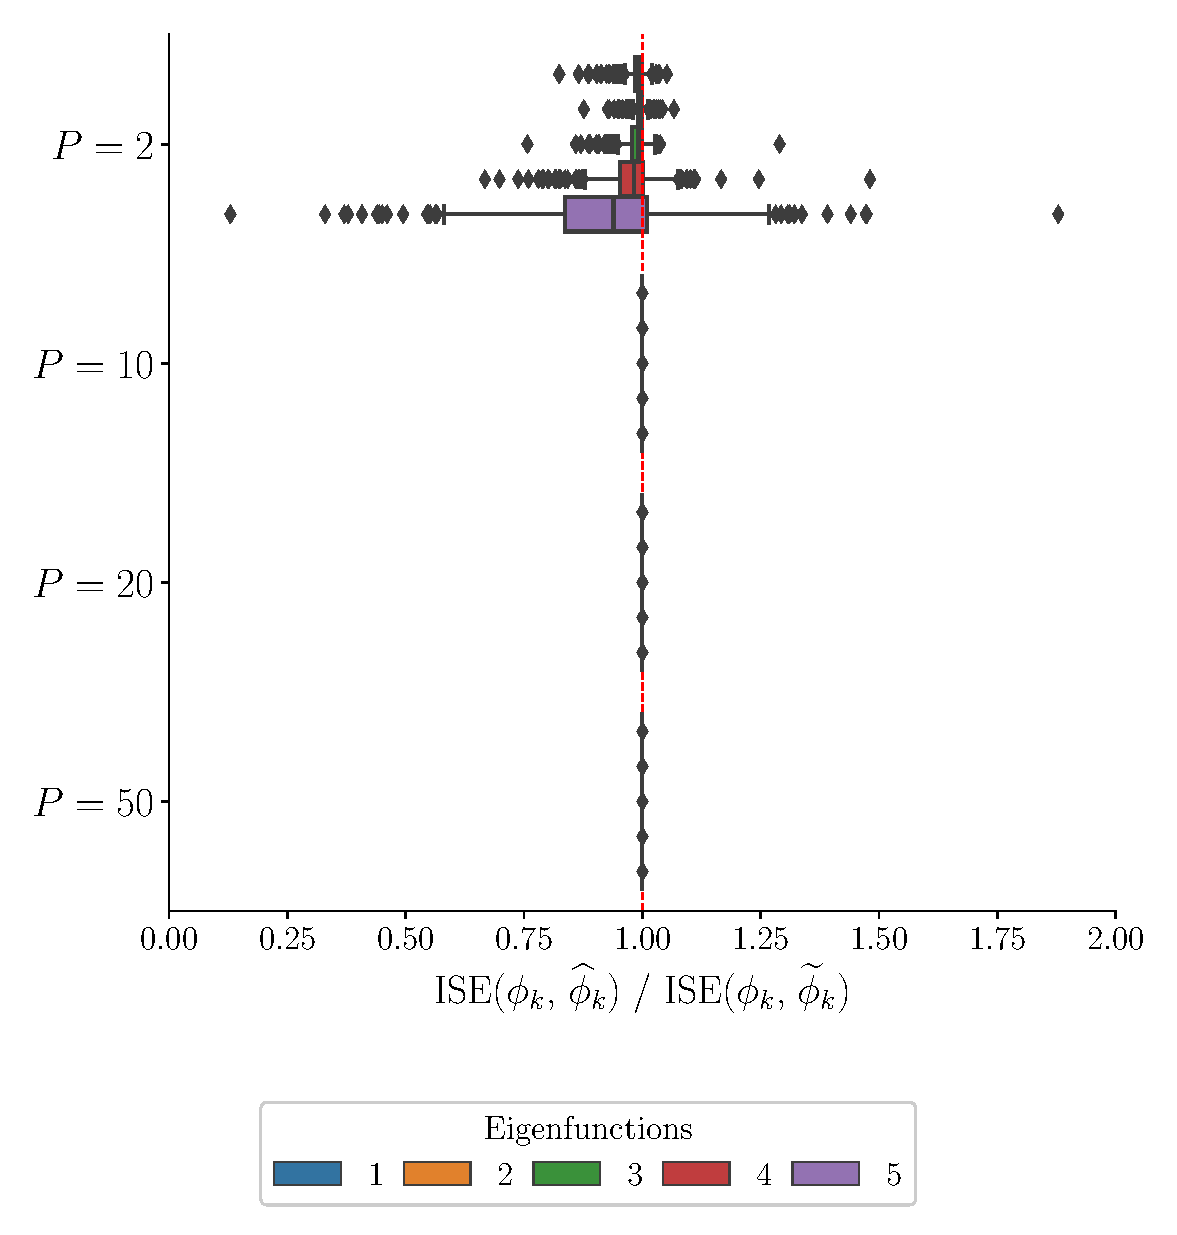
\includegraphics[width=\textwidth]{figures/scenario_1/ise_N50_M100.eps}
         \caption{$M = 100$}
         \label{fig:ise_mfd_1d_100}
    \end{subfigure}
    \caption{ISE for multivariate functional data. Each univariate component is defined on a one-dimensional domain. We simulated $N = 50$ observations for each dataset.}
    \label{fig:ise_mfd_1d}
\end{figure}

\begin{figure}
     \centering
     \begin{subfigure}[b]{0.49\textwidth}
         \centering
         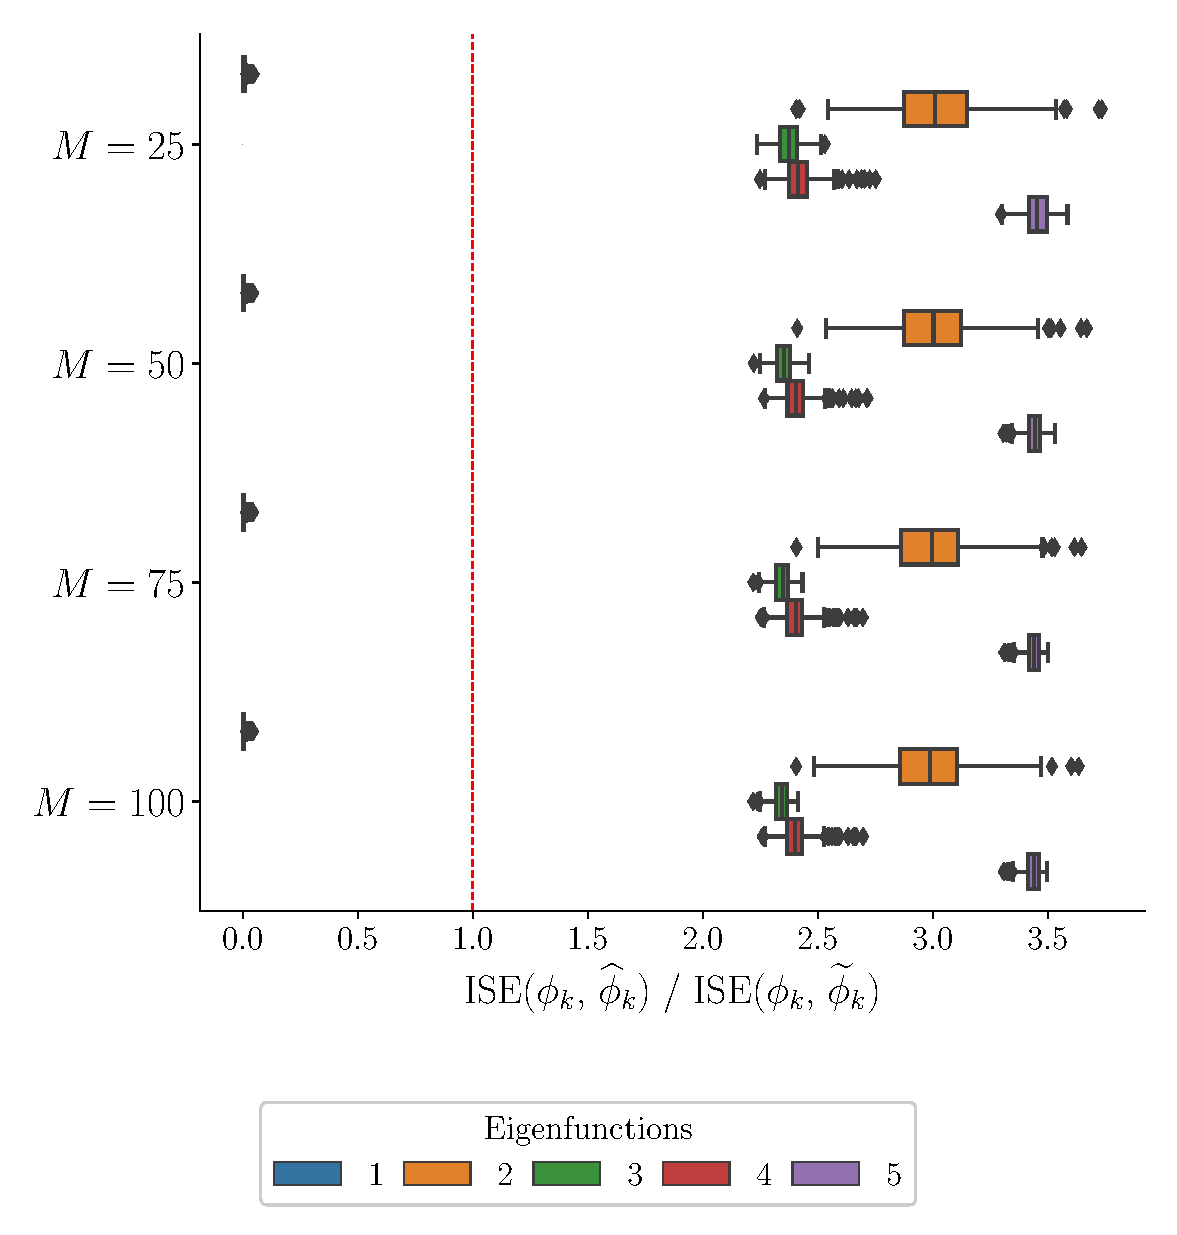
\includegraphics[width=\textwidth]{figures/scenario_2/ise_N25.eps}
         \caption{$N = 25$}
         \label{fig:ise_mfd_2d_25}
     \end{subfigure}
     \hfill
     \begin{subfigure}[b]{0.49\textwidth}
         \centering
         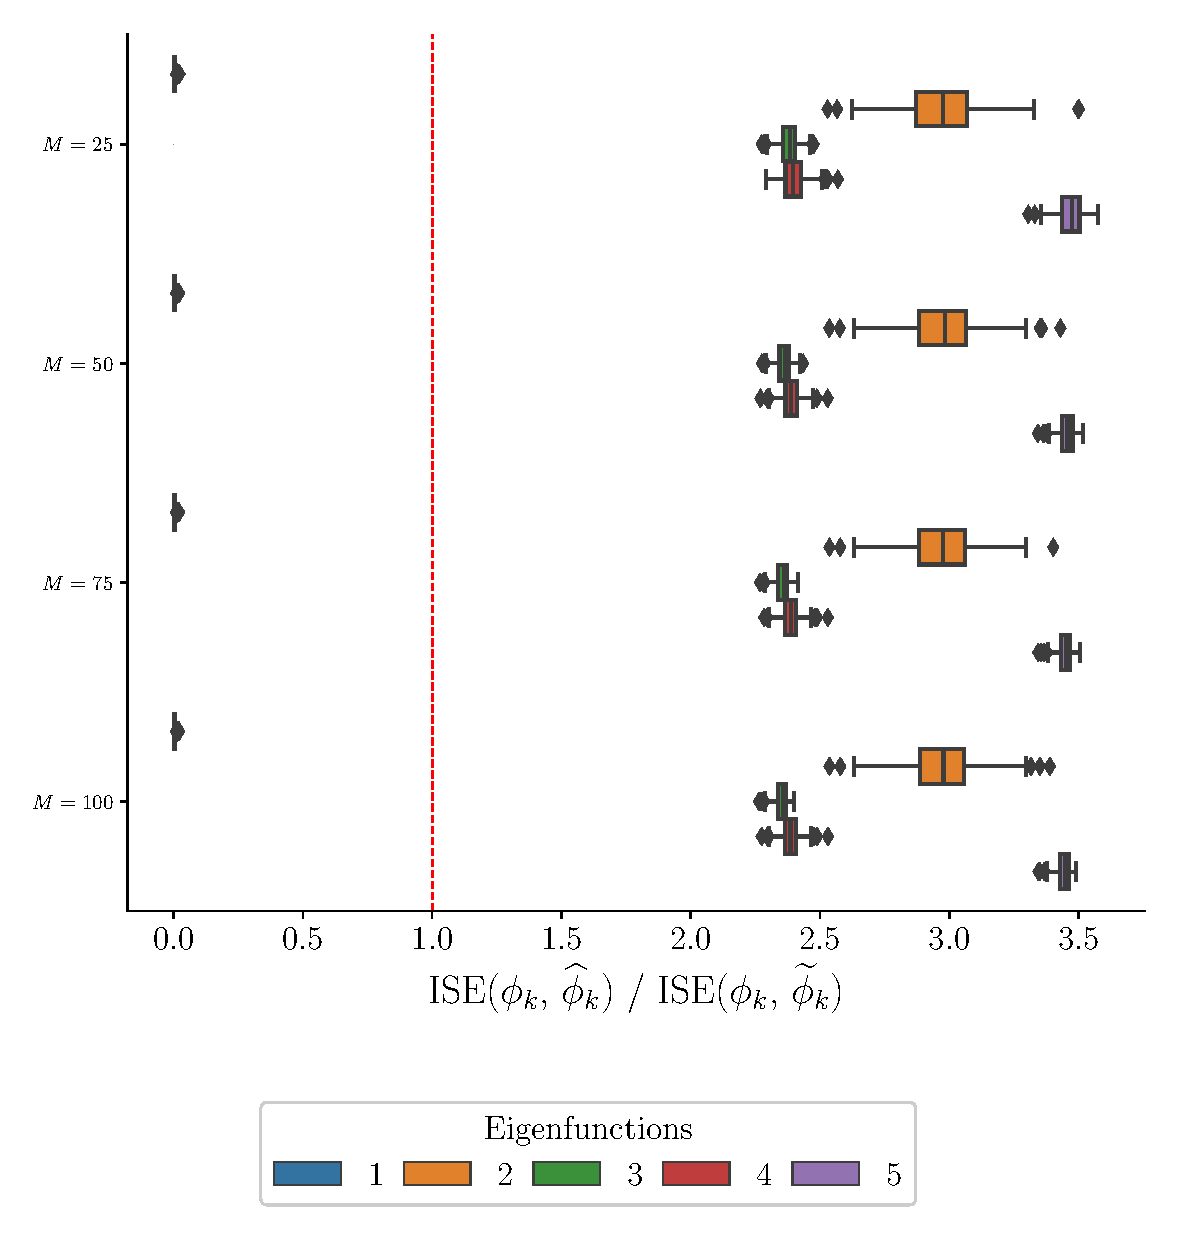
\includegraphics[width=\textwidth]{figures/scenario_2/ise_N50.eps}
         \caption{$N = 50$}
         \label{fig:ise_mfd_2d_50}
     \end{subfigure}
     \\
     \begin{subfigure}[b]{0.49\textwidth}
         \centering
         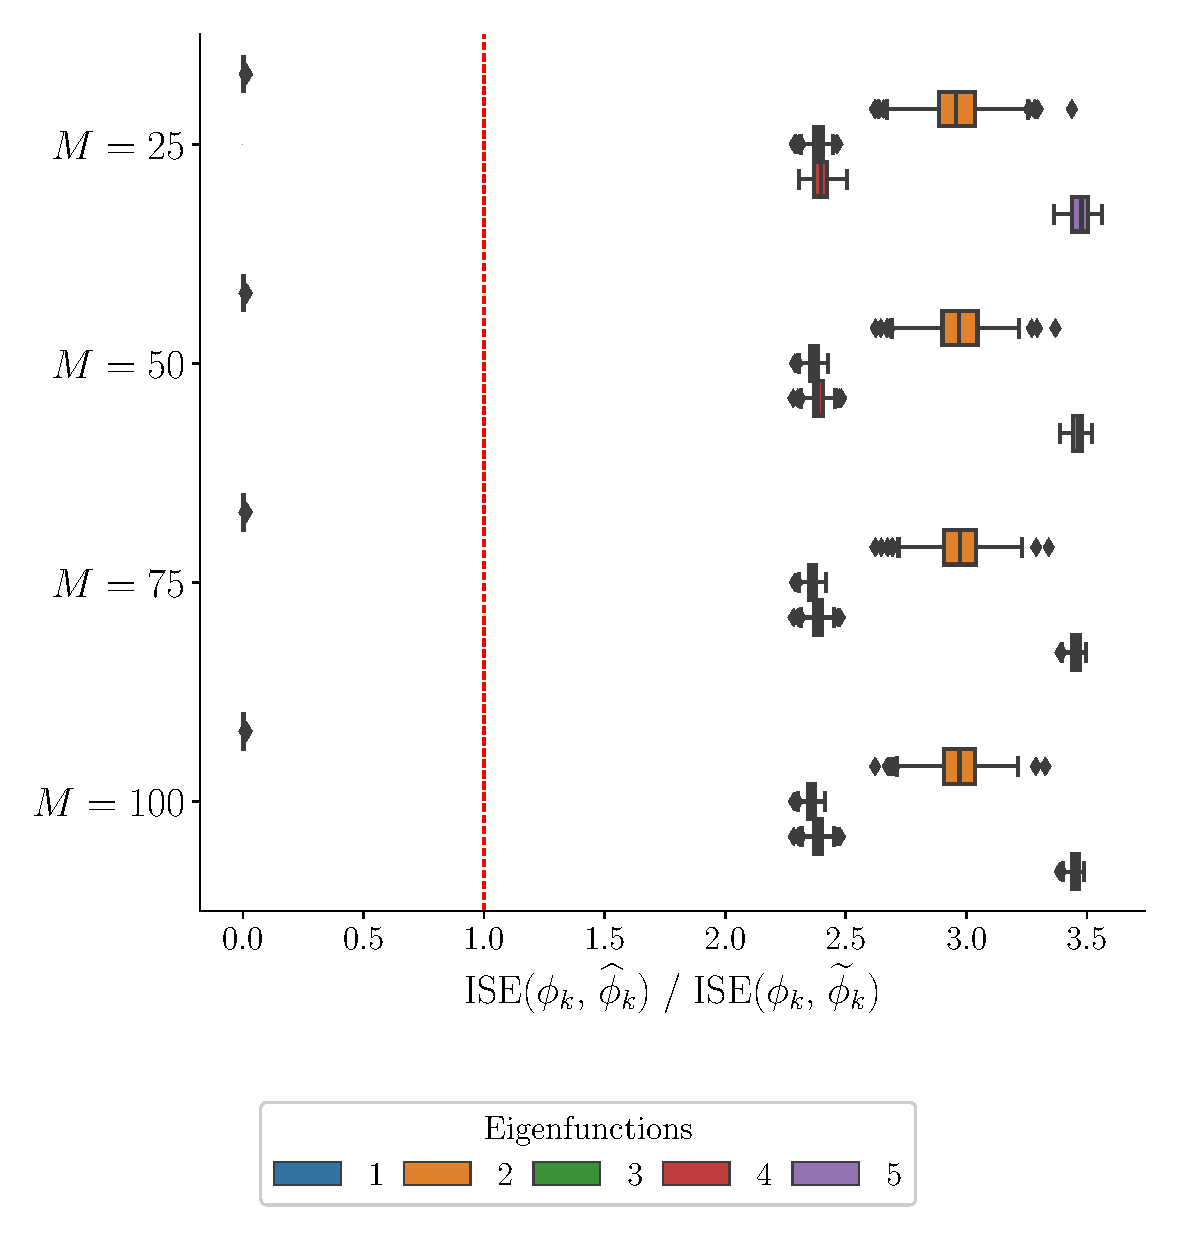
\includegraphics[width=\textwidth]{figures/scenario_2/ise_N75.eps}
         \caption{$N = 75$}
         \label{fig:ise_mfd_2d_75}
     \end{subfigure}
     \begin{subfigure}[b]{0.49\textwidth}
         \centering
         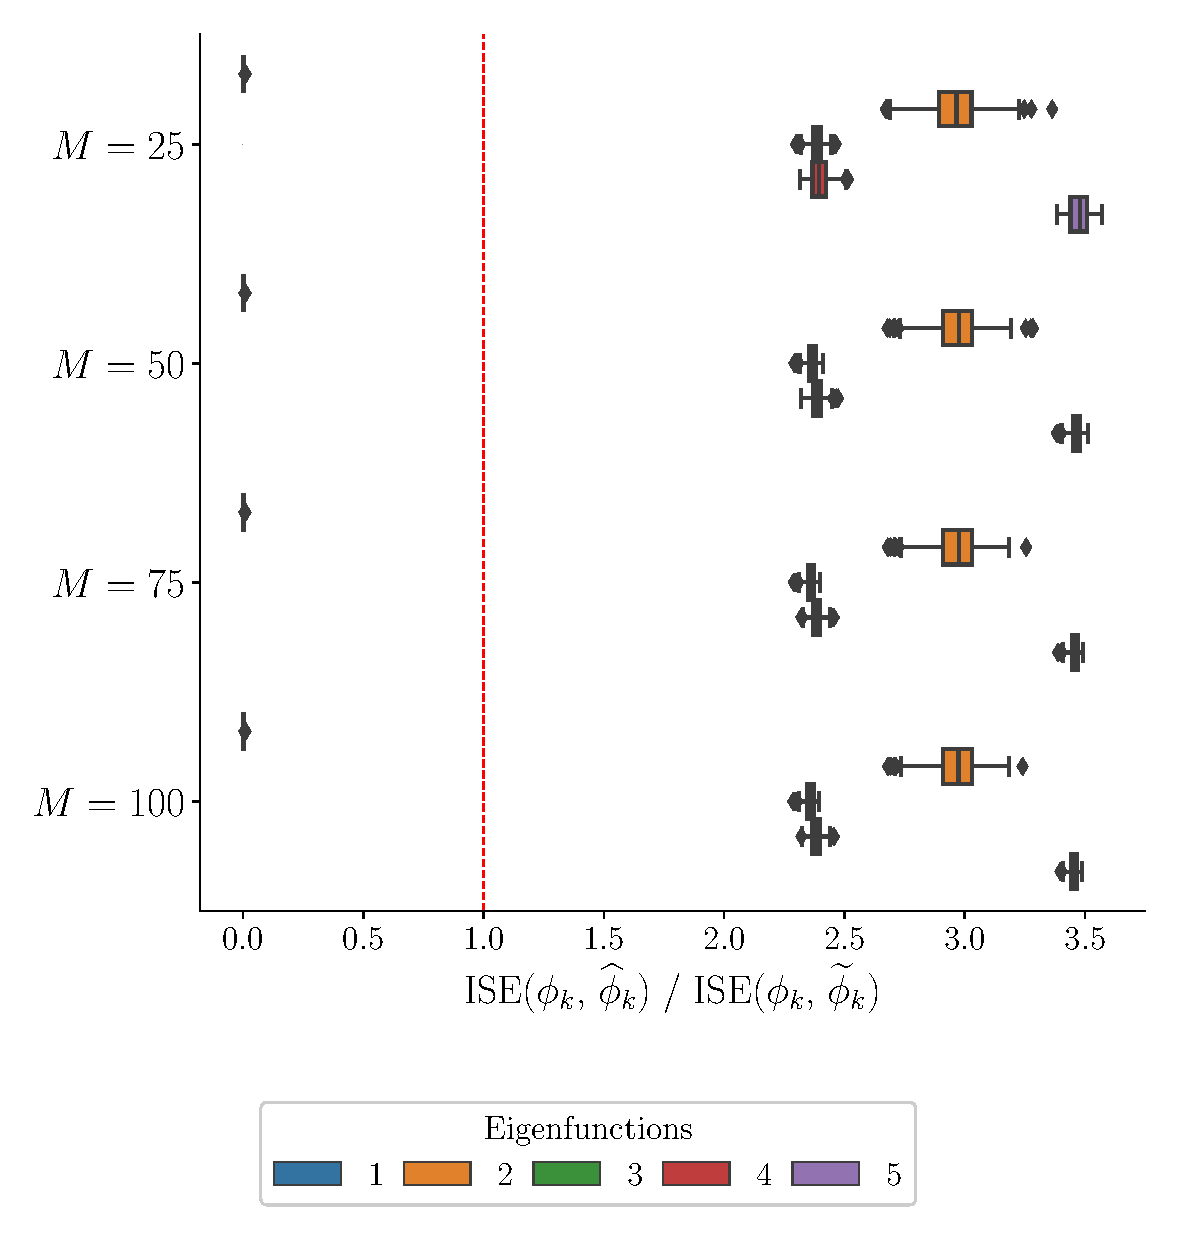
\includegraphics[width=\textwidth]{figures/scenario_2/ise_N100.eps}
         \caption{$N = 100$}
         \label{fig:ise_mfd_2d_100}
    \end{subfigure}
    \caption{ISE for univariate functional data of images data}
    \label{fig:ise_mfd_2d}
\end{figure}

\end{results}

% Curves reconstruction ----------
\begin{results}[Curves reconstruction]

Figure~\ref{fig:mise_mfd_1d} and Figure~\ref{fig:mise_mfd_2d}.

\begin{figure}
     \centering
     \begin{subfigure}[b]{0.49\textwidth}
         \centering
         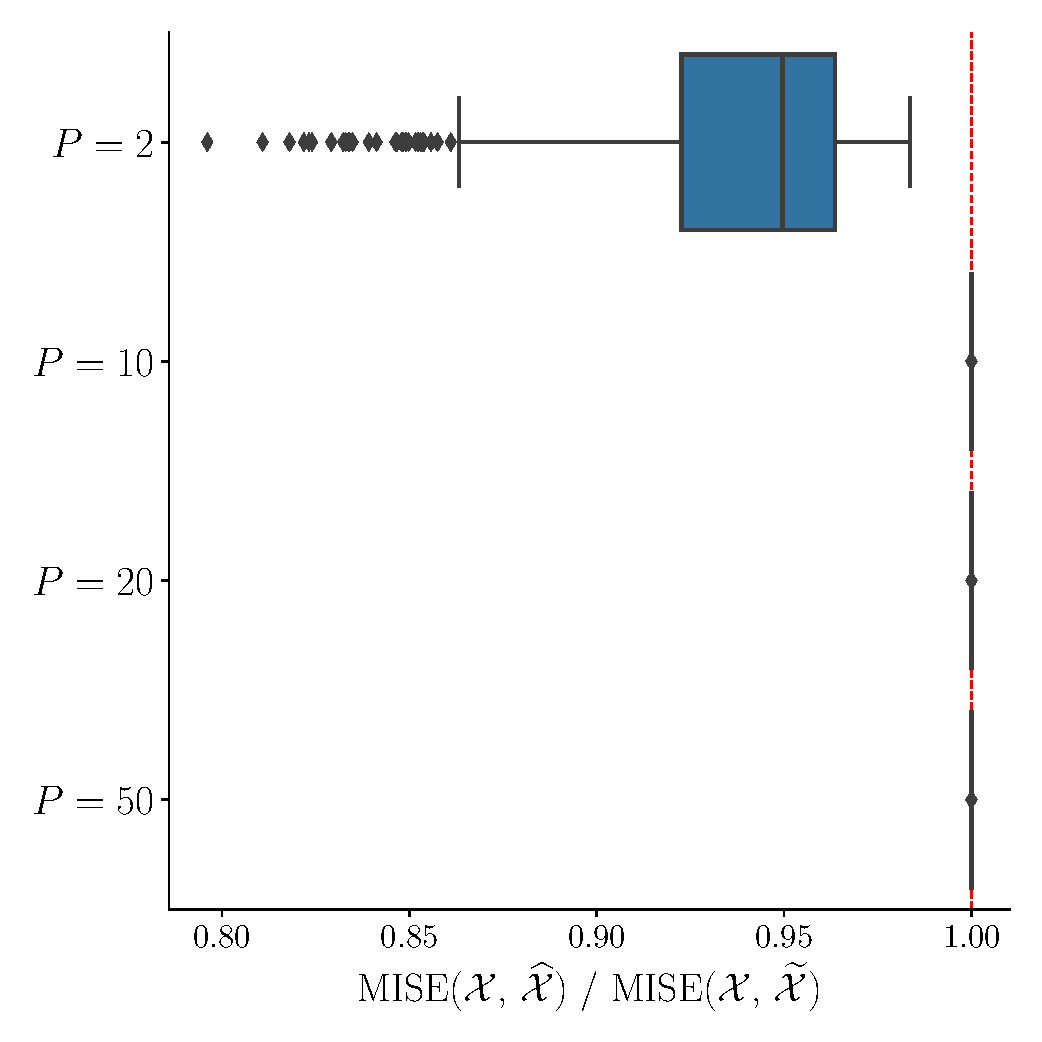
\includegraphics[width=\textwidth]{figures/scenario_1/mise_N50_M25.eps}
         \caption{$M = 25$}
         \label{fig:mise_mfd_1d_25}
     \end{subfigure}
     \hfill
     \begin{subfigure}[b]{0.49\textwidth}
         \centering
         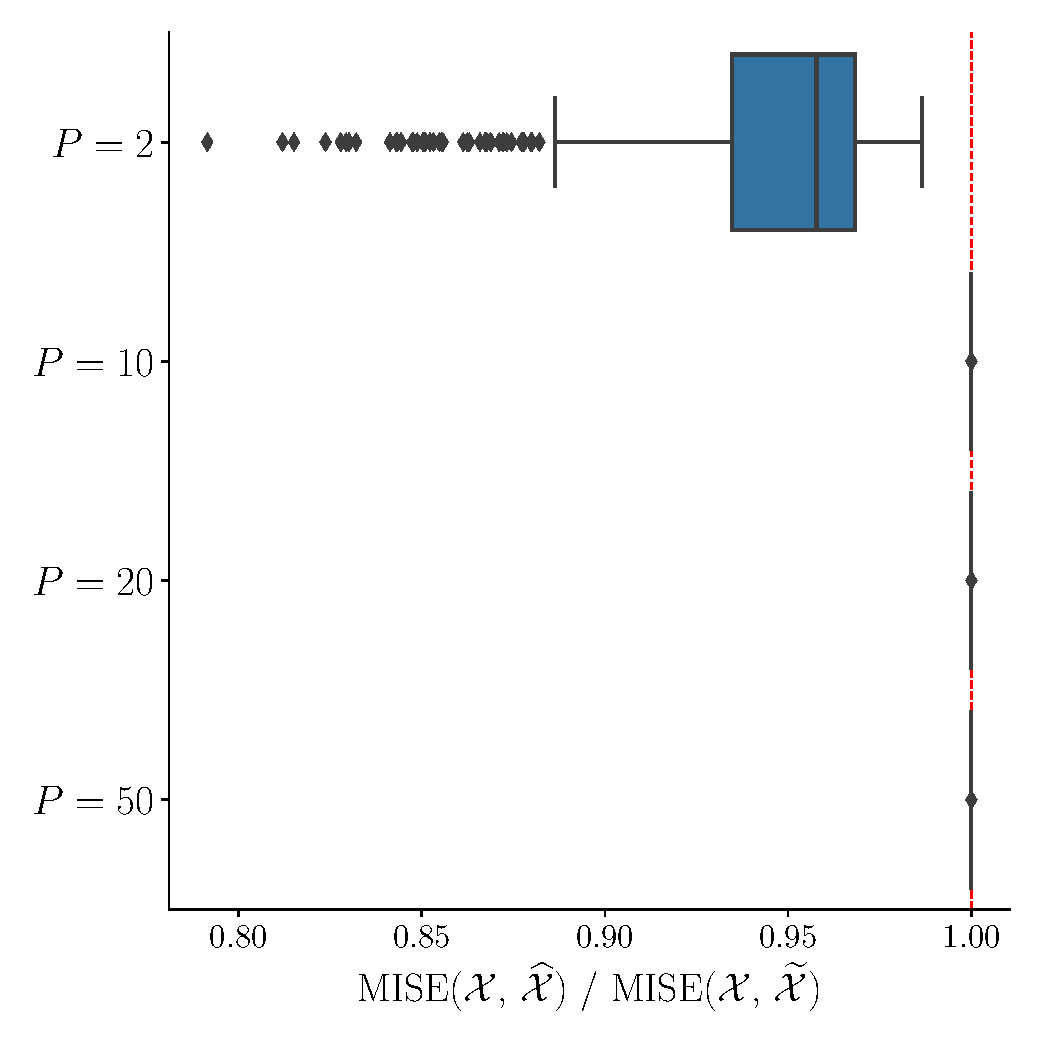
\includegraphics[width=\textwidth]{figures/scenario_1/mise_N50_M50.eps}
         \caption{$M = 50$}
         \label{fig:mise_mfd_1d_50}
     \end{subfigure}
     \\
     \begin{subfigure}[b]{0.49\textwidth}
         \centering
         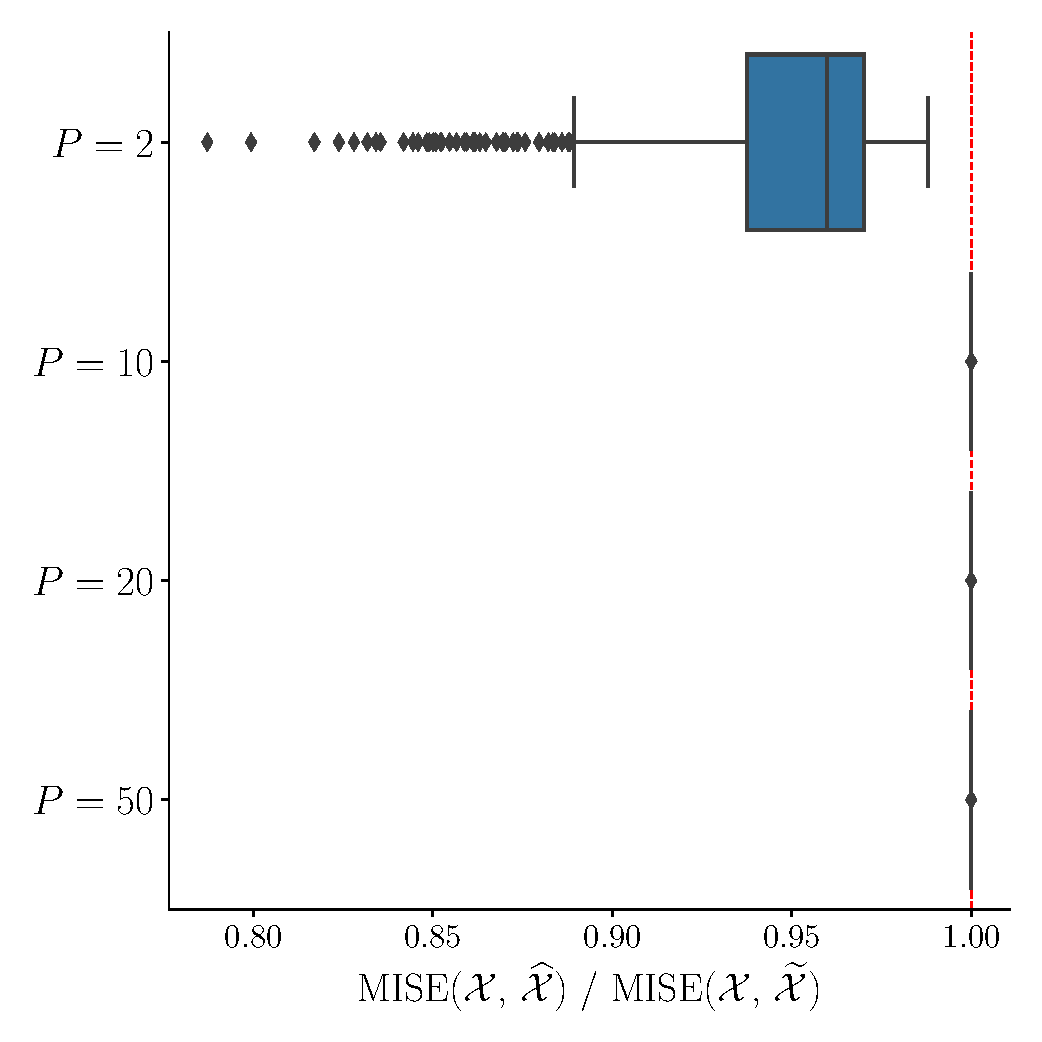
\includegraphics[width=\textwidth]{figures/scenario_1/mise_N50_M75.eps}
         \caption{$M = 75$}
         \label{fig:mise_mfd_1d_75}
     \end{subfigure}
     \begin{subfigure}[b]{0.49\textwidth}
         \centering
         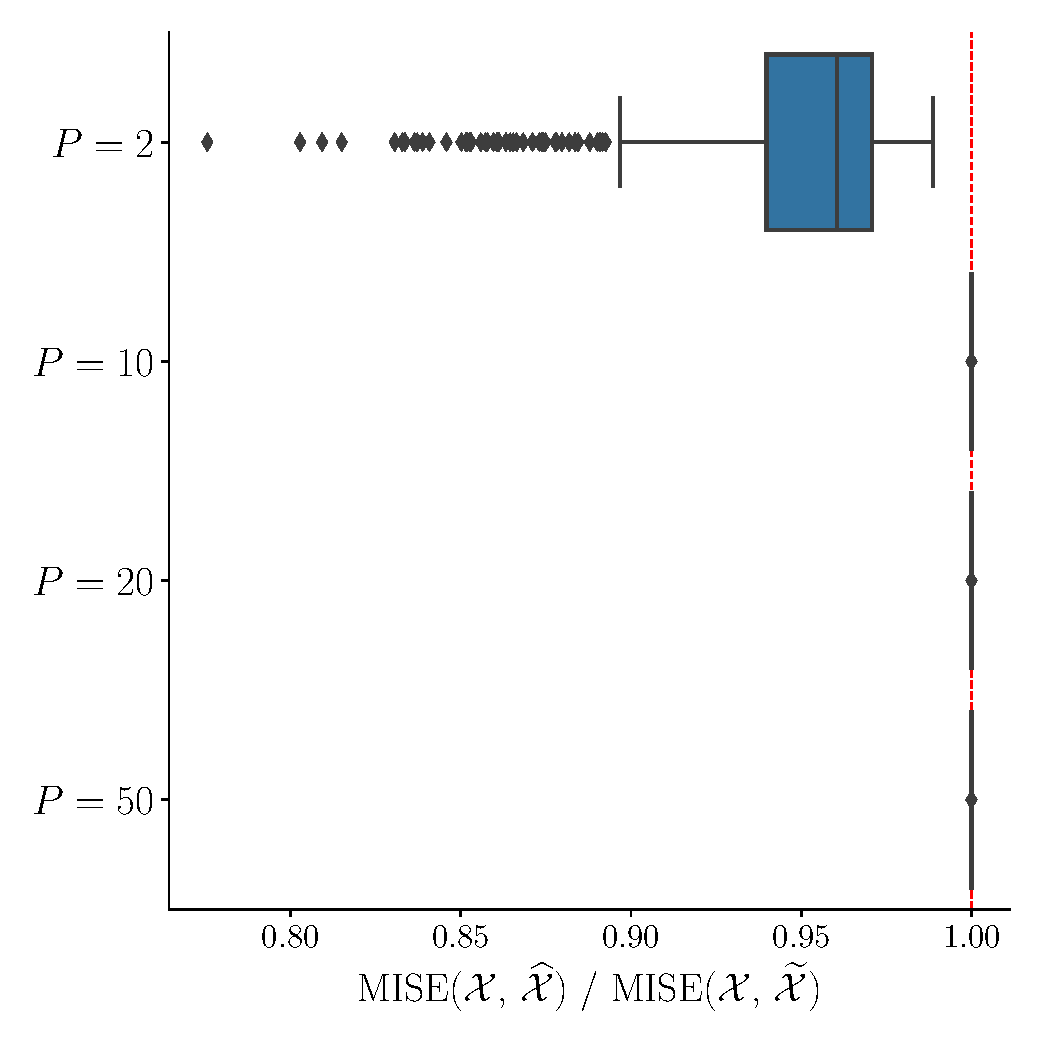
\includegraphics[width=\textwidth]{figures/scenario_1/mise_N50_M100.eps}
         \caption{$M = 100$}
         \label{fig:mise_mfd_1d_100}
    \end{subfigure}
    \caption{MISE for multivariate functional data. Each univariate component is defined on a one-dimensional domain. We simulated $N = 50$ observations for each dataset.}
    \label{fig:mise_mfd_1d}
\end{figure}

\begin{figure}
     \centering
     \begin{subfigure}[b]{0.49\textwidth}
         \centering
         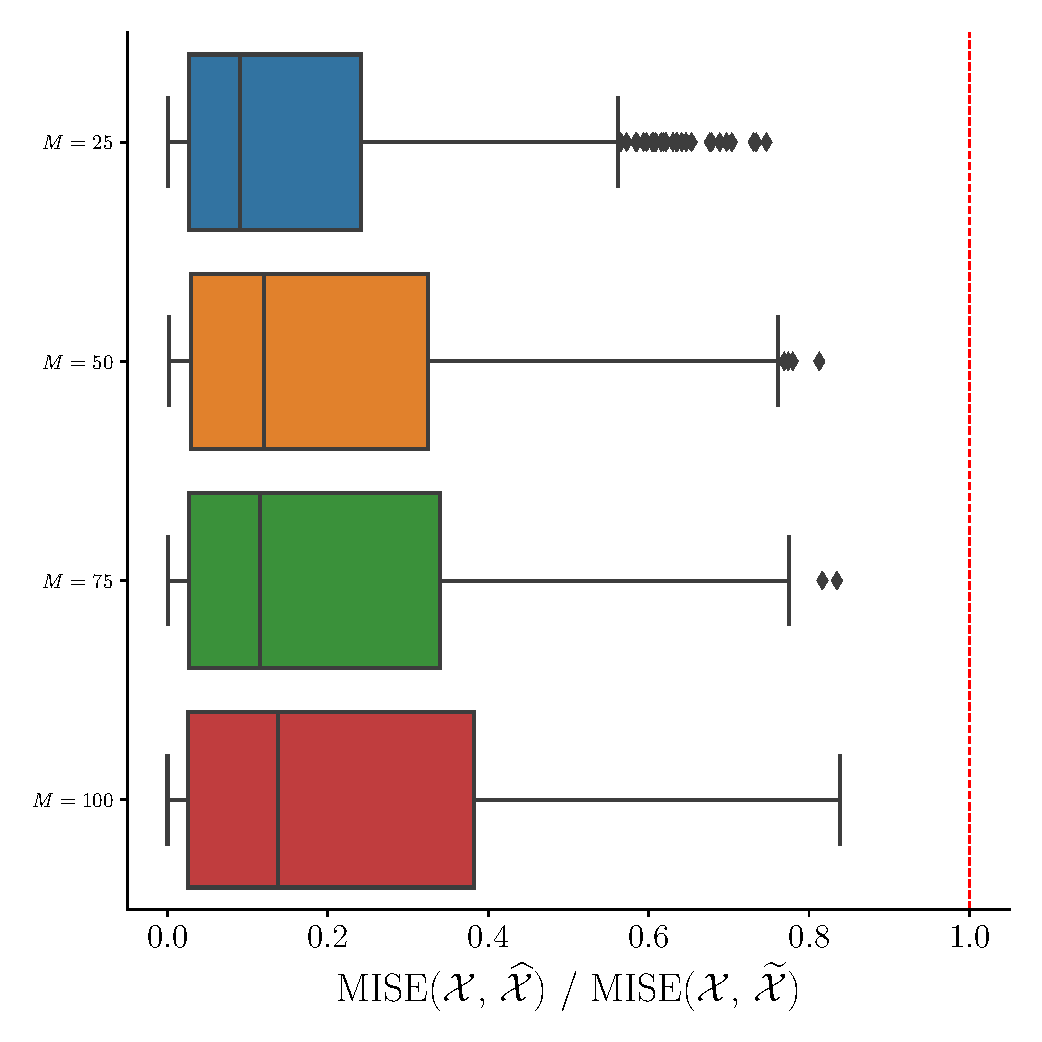
\includegraphics[width=\textwidth]{figures/scenario_2/mise_N25.eps}
         \caption{$N = 25$}
         \label{fig:mise_mfd_2d_25}
     \end{subfigure}
     \hfill
     \begin{subfigure}[b]{0.49\textwidth}
         \centering
         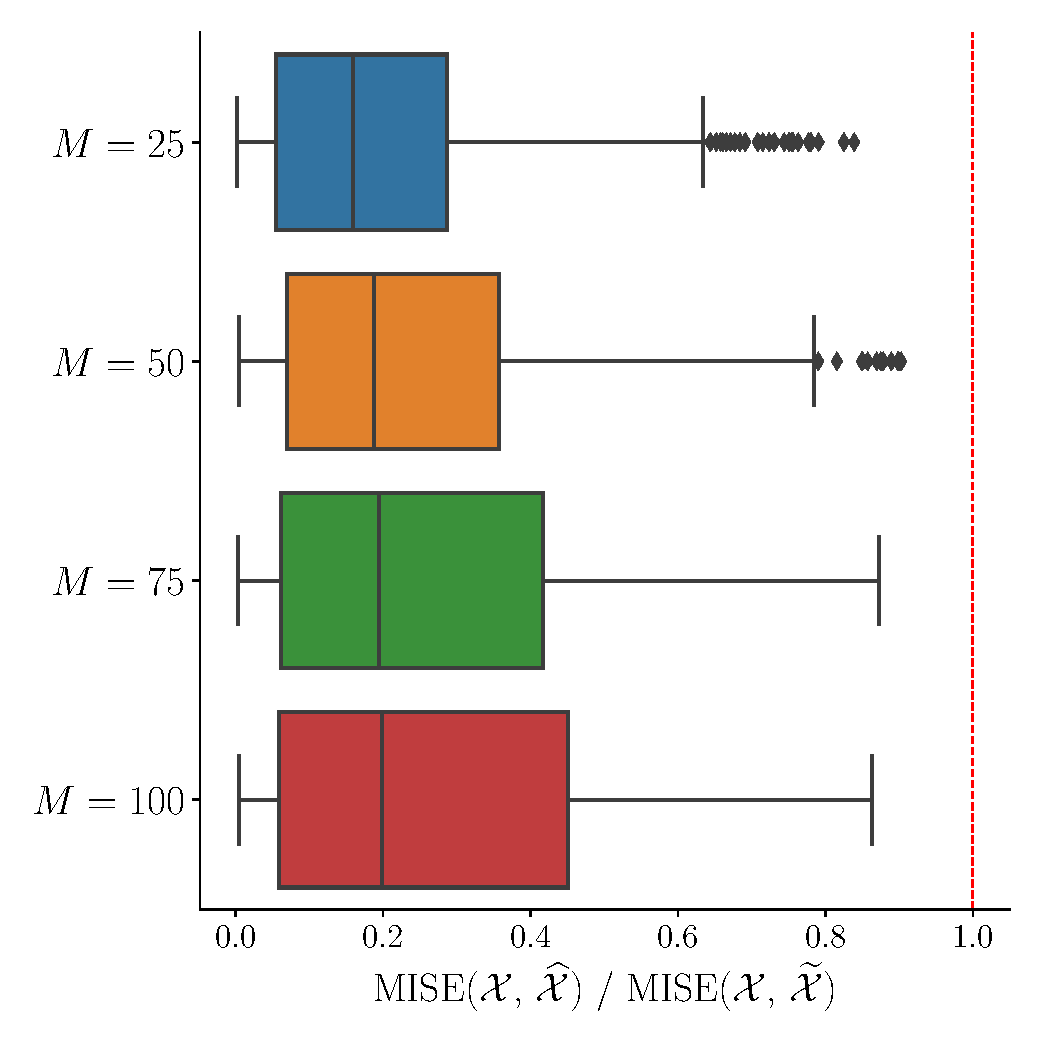
\includegraphics[width=\textwidth]{figures/scenario_2/mise_N50.eps}
         \caption{$N = 50$}
         \label{fig:mise_mfd_2d_50}
     \end{subfigure}
     \\
     \begin{subfigure}[b]{0.49\textwidth}
         \centering
         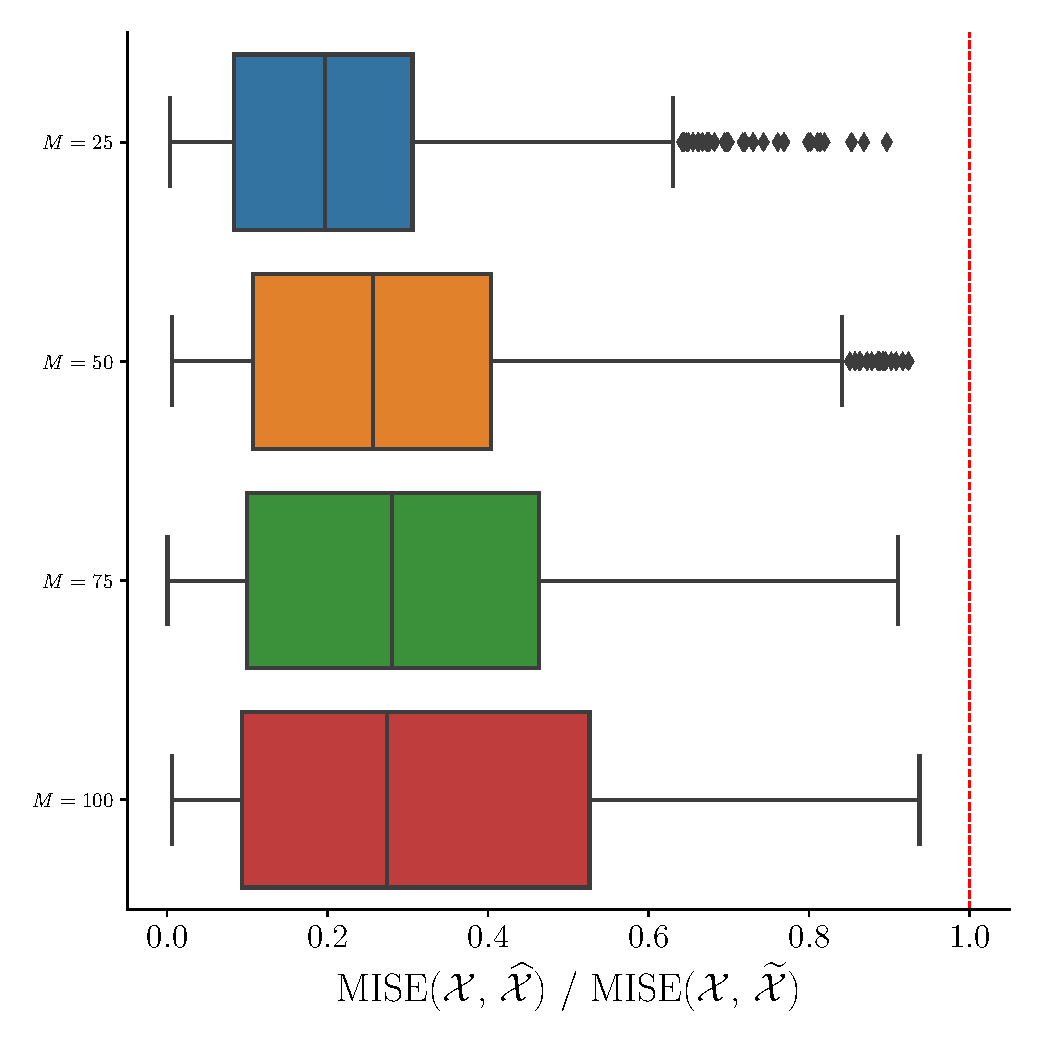
\includegraphics[width=\textwidth]{figures/scenario_2/mise_N75.eps}
         \caption{$N = 75$}
         \label{fig:mise_mfd_2d_75}
     \end{subfigure}
     \begin{subfigure}[b]{0.49\textwidth}
         \centering
         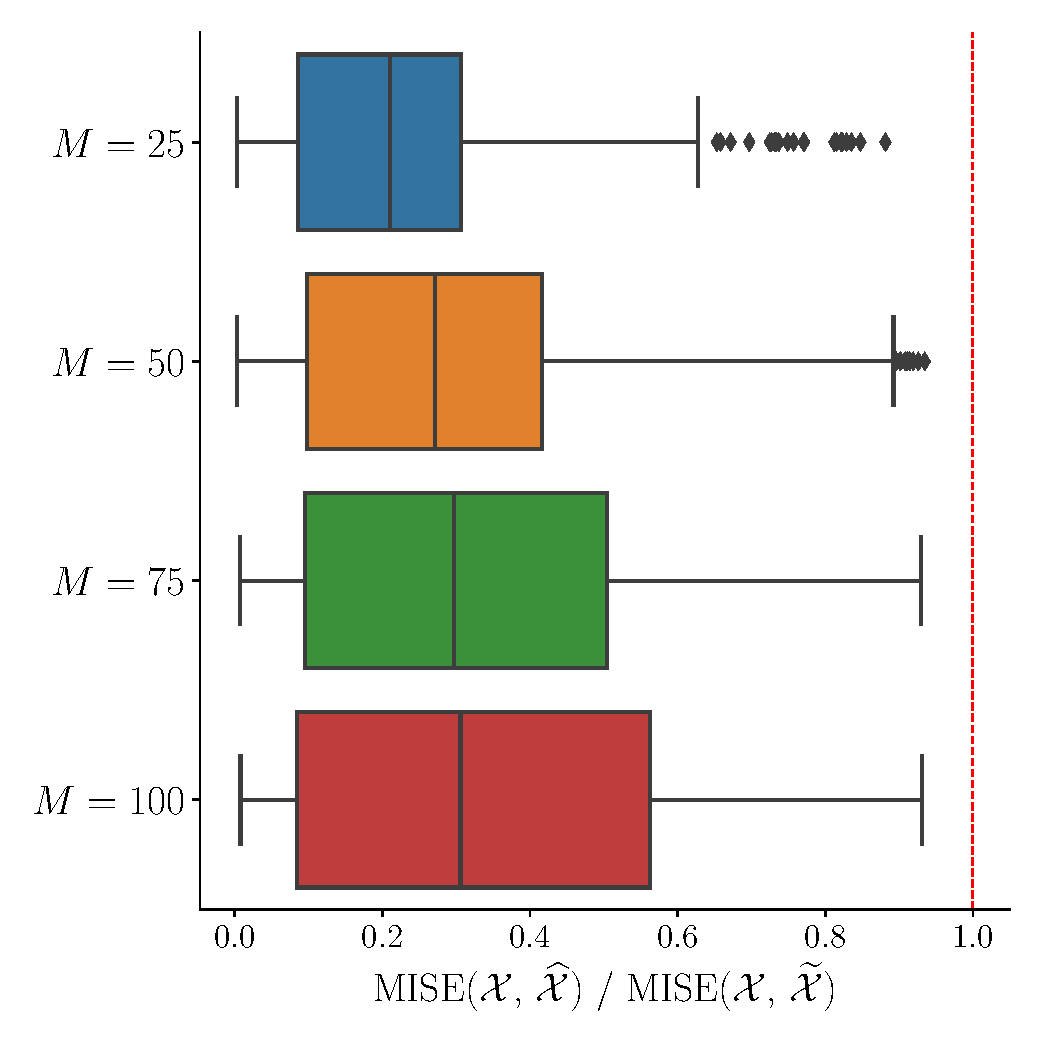
\includegraphics[width=\textwidth]{figures/scenario_2/mise_N100.eps}
         \caption{$N = 100$}
         \label{fig:mise_mfd_2d_100}
    \end{subfigure}
    \caption{MISE for univariate functional data of images data}
    \label{fig:mise_mfd_2d}
\end{figure}

\end{results}


% subsection simulation_results (end)

\subsection{Percentage of variance explained} % (fold)
\label{sub:percentage_of_variance_explained_simulation}

\textcolor{red}{We argue that the percentage of variance explained in \cite{happMultivariateFunctionalPrincipal2018a} is not the good one as they consider the variance explained by each of the components separately and not as a all. Using the inner product matrix however gives the right number of eigenfunctions for a given amount of variance explained.
We also consider the estimation of the number of components to retain to reach a prespecify percentage of variance explained by the data based on the Scenario~1 with $P = 2$, $K = 20$ and we use linear and exponential decreasing of the eigenvalues. The true percentage of variance explained by the $k$th component is given by $\lambda_k / \sum_{k^\prime = 1}^{20} \lambda_{k^\prime}$ and the true percentage of variance explained by the first $K (\leq 20)$ components is given by $\sum_{k = 1}^K \lambda_k / \sum_{k^\prime = 1}^{20} \lambda_{k^\prime}$.
Let fix a certain percentage of variance explained $\alpha \in [0, 1]$. We define $\widetilde{K}$ as the minimum number of components to estimate to reach $100\alpha\%$ of the variance explained,
\begin{equation}
    \widetilde{K} = \arg\min_K \frac{\sum_{k = 1}^K \lambda_k}{\sum_{k^\prime = 1}^{20} \lambda_{k^\prime}} \geq \alpha.
\end{equation}
Using the covariance operator, the implementation of \cite{happMultivariateFunctionalPrincipal2018a} does not allow to directly estimated $\widetilde{K}$ from the multivariate functional data. They propose however to estimate the number of univariate eigenfunctions $K_1$ and $K_2$ based on the percentage of variance explained $\alpha$ for both elements. The number of multivariate eigenfunctions is then set to be $\min\{K_1 + K_2, K\}$ where $K$ is a given scalar. In the simulation, we first run FPCA on each univariate components to estimate the number of components needed to explain $\alpha\%$ of the variance for each components. Then, we run an MFPCA with $K = K_1 + K_2$. Using the Gram matrix, we directly estimated the number of components needed to explain a certain percentage of the variance from the multivariate functional data.
It seems to show that choosing a univariate cut-off within each dimension (e.g., $95\%$), tends to overestimate the final amount of variance – the sum of the final eigenvalues is larger than the sum of the true eigenvalues.}


% subsection percentage_of_variance_explained (end)

% section empirical_analysis (end)